%
%     Hauptdatei des Latex-Dokuments
%
%
%========================= Allgemeine Informationen =============================
% Angaben zum Autor, der Arbeit und dem Betreuer
\def \AUTHOR     {Viviane Bremer, Justus Dr�gem�ller, Manish Kumar} 
\def \TITLE      {Fachlabor Mikromechatronik}
\def \TYPE       {Laborprotokoll}
\def \MATRIKELNR {4254652, 4427984, 4847551}
%\def \BETREUER   {Dipl.-Ing. Vor- und Zuname}
%==================== Ende allgemeine Informationen =============================



%
%		Header-Datei
%

\documentclass[
	pdftex,             % Ausgabe des Latex-Dokuments als PDF
	12pt,				        % Schriftgroesse 12pt
	a4paper,		      	% Layout fuer Din A4
	german,			      	% deutsche Sprache, global
	BCOR10mm,		        % DIV-Wert fuer die Erstellung des Satzspiegels
	DIV14,				      % Korrektur f�r die Bindung
	parskip=half,       % Absatzgr��e -> halber Zeilenabstand
	oneside,			      % Einseitiger Druck
	%twoside,		        % Zweiseitiger Druck
	openany,            % Kapitel k�nnen auf geraden und ungeraden Seiten beginnen
	numbers=noenddot,   % Kapitelnummern immer ohne Punkt
	bibliography=totoc,	% Literaturverzeichnis im Inhaltsverzeichnis angeben
	index=totoc			    % Index im Inhaltsverzeichnis angeben
]{scrreprt}


% PDF-Dokument formatieren
\usepackage[
	pdftitle={\TITLE},
	pdfauthor={\AUTHOR},
	pdfcreator={pdfLatex},
	pdfsubject={\TYPE\ am Institut f�r Mikrotechnik der Technischen Universit�t Braunschweig},
	pdfkeywords={\TYPE, Technische Universit�t Braunschweig, TU-BS, Institut f�r Mikrotechnik, IMT, \TITLE, \AUTHOR, \MATRIKELNR},
  colorlinks={true}, % Umrandung von Links nicht sichtbar
  linkcolor={black},
  citecolor={black},
  filecolor={black},
  urlcolor={black},
	pdflang={de},
	hyperindex=true
]{hyperref}

% Deutsche Rechtschreibung
\usepackage{german,ngerman}
\usepackage[latin1]{inputenc}
\usepackage[T1]{fontenc}
\usepackage{lmodern}		%Schriftart
\usepackage[all]{nowidow}		%Hurenkinder+Schusterjungen unterdr�cken

% Aktuelles Datum ermitteln
\usepackage[ngerman]{datenumber}

% Erweiterung f�r ein deutsches Literaturverzeichnis
\bibliographystyle{alphadin}

% Benutzerdefinierte Kopf- und Fu�zeile
\usepackage[automark]{scrpage2}
\pagestyle{scrheadings}
\setheadsepline{.4pt} % Linie unter dem Header

% Erweiterte Mathematikbibliotheken
\usepackage{siunitx}
\usepackage{amsmath}
\usepackage{amssymb}

% Ma�einhaeiten-Darstellung verbessern
\usepackage{units}

%Sch�nere Tabellen
\usepackage[table,xcdraw]{xcolor}
\usepackage{booktabs}	
\usepackage{tabularx}	%Zeilenumbruch und automatische Breiteneinstellung in Tabellen
\usepackage{longtable}	%lange Tabellen mit Seitenumbruch
\usepackage{multirow}	%Zellen verbinden

% Einbinden von externen PDF Dateien
\usepackage[final]{pdfpages}

% Zum einbinden von Grafiken 
\usepackage{float} 
\usepackage{graphicx}
\usepackage{subfigure}

                         % Latex-Packages und Layout Konfiguration

\usepackage{pgfplots}

\usepgfplotslibrary{groupplots}
\usepackage{pgfplotstable}
\pgfplotsset{compat=1.15}
%\usetikzlibrary{datavisualization}
%\usetikzlibrary{datavisualization.formats.functions}
 \usetikzlibrary{plotmarks}
%Einstellen des plots
\pgfplotsset{every axis/.append style={thick}}
\pgfplotsset{every axis title/.style={
		inner sep=3pt,
		at={(0.03,1)},anchor=north west,
		yshift=-3pt,xshift=-3pt,
		fill=white,}}
\pgfplotsset{every axis legend/.append style={
		draw=none, 
		legend columns=3, 
		at={(0.5,1)}, 
		anchor=south,
		legend cell align=left}}
	

\definecolor{color1}{RGB}{27,158,119}
\definecolor{color2}{RGB}{217,95,2}
\definecolor{color3}{RGB}{117,112,179}
\definecolor{color4}{RGB}{231,41,138}
%\pgfplotscreateplotcyclelist{mylist}{%
%	{color1, solid ,mark=*},
%	{color2, densely dashed,mark=square*},
%	{color3, densely dotted,mark=triangle*}}

\pgfplotsset{every mark/.append style={solid,mark=x}} % damit marker alle solid

\pgfplotsset{major grid style={dotted,black!30!white}}	

\pgfplotsset{every axis/.append style={
%		xtick={-0,0.1,...,1.1},
		mark=x,
		xtick distance=0.1,
		major tick style={semithick,color=gray},
		minor tick style={thin, color=gray},
%		minor tick num=1,
		grid=major,
		footnotesize,
		xlabel=p / bar,
		scale only axis,
		height=8cm,
		width=0.8\textwidth, %width=11.3cm,
%		xmin=-1,xmax=8,
		unbounded coords=jump, %skip
}}

\pgfplotsset{every axis/.append style={ %europaeische Darstellung der Zahlen
		/pgf/number format/.cd,
		use comma,
		1000 sep={},
}}
	

\makeatletter
% #1: keys
\def\pgfplotstable@linear@regression#1{%
    \begingroup
    \pgfqkeys{/pgfplots/table/create col/linear regression}{/pgf/fpu,#1}%
    \pgfkeysgetvalue{/pgfplots/table/create col/linear regression/x}{\pgfplotstable@xsrc}%
    \pgfkeysgetvalue{/pgfplots/table/create col/linear regression/y}{\pgfplotstable@ysrc}%
    \pgfkeysgetvalue{/pgfplots/table/create col/linear regression/table}{\pgfplotstable@table}%
    \pgfkeysgetvalue{/pgfplots/table/create col/linear regression/xmode}{\pgfplotstable@xmode}%
    \pgfkeysgetvalue{/pgfplots/table/create col/linear regression/ymode}{\pgfplotstable@ymode}%
    \pgfkeysgetvalue{/pgfplots/table/create col/linear regression/variance}{\pgfplotstable@variance@colname}%
    \pgfkeysgetvalue{/pgfplots/table/create col/linear regression/variance list}{\pgfplotstable@variance@list}%
    \pgfkeysgetvalue{/pgfplots/table/create col/linear regression/variance src}{\pgfplotstable@variance@table}%
    %
    \ifx\pgfplotstable@table\pgfutil@empty
        \pgfutil@ifundefined{pgfplotstablename}{}{% query the name of the actual table struct
            \let\pgfplotstable@table=\pgfplotstablename
        }%
    \fi
    \ifx\pgfplotstable@table\pgfutil@empty
        \pgfplots@error{Sorry, I couldn't determine a value for create col/linear regression/table. Which table should I load?}%
    \fi
    \ifx\pgfplotstable@xsrc\pgfutil@empty
        \pgfplotsifinaddplottablestruct{%
            \pgfutil@ifundefined{pgfplots@plot@tbl@x}{}{%
                \let\pgfplotstable@xsrc=\pgfplots@plot@tbl@x
                \ifx\pgfplotstable@ysrc\pgfutil@empty
                    \pgfplotstablegetcolsof\pgfplots@table
                    \ifnum\pgfplotsretval=2
                    \else
                        \pgfplotsthrow{invalid argument}{\pgfplotstable@ysrc}{Sorry, I don't which column should be used as `y' for the linear regression. Please provide 'linear regression={y=<colname>}'}\pgfeov%
                    \fi
                \fi
            }%
        }{}%
    \fi
    \ifx\pgfplotstable@xsrc\pgfutil@empty
        \def\pgfplotstable@xsrc{[index]0}%
    \fi
    \ifx\pgfplotstable@ysrc\pgfutil@empty
        \def\pgfplotstable@ysrc{[index]1}%
    \fi
    %
    \t@pgfplots@toka=\expandafter{\pgfplotstable@table}%
    \t@pgfplots@tokb=\expandafter{\pgfplotstable@xsrc}%
    \t@pgfplots@tokc=\expandafter{\pgfplotstable@ysrc}%
    \edef\pgfplots@loc@TMPa{{\the\t@pgfplots@tokb}\noexpand\of{\the\t@pgfplots@toka}}%
    \edef\pgfplots@loc@TMPb{{\the\t@pgfplots@tokc}\noexpand\of{\the\t@pgfplots@toka}}%
    \expandafter\pgfplotstablegetcolumn\pgfplots@loc@TMPa\to\pgfplotstable@X
    \expandafter\pgfplotstablegetcolumn\pgfplots@loc@TMPb\to\pgfplotstable@Y
    %
    \edef\pgfplotstable@xmode{\pgfplotstable@xmode}%
    \expandafter\pgfplotstable@linear@regression@prepare@mode\expandafter{\pgfplotstable@xmode}{x}%%
    \edef\pgfplotstable@ymode{\pgfplotstable@ymode}%
    \expandafter\pgfplotstable@linear@regression@prepare@mode\expandafter{\pgfplotstable@ymode}{y}%%
    %
    \ifx\pgfplotstable@variance@list\pgfutil@empty
        % check 'variance' key (loaded from table)
        \pgfplotslistnewempty\pgfplotstable@VARIANCE
        \ifx\pgfplotstable@variance@colname\pgfutil@empty
        \else
            \ifx\pgfplotstable@variance@table\pgfutil@empty
                \t@pgfplots@toka=\expandafter{\pgfplotstable@table}%
                \t@pgfplots@tokb=\expandafter{\pgfplotstable@variance@colname}%
                \edef\pgfplots@loc@TMPa{{\the\t@pgfplots@tokb}\noexpand\of{\the\t@pgfplots@toka}}%
                \expandafter\pgfplotstablegetcolumn\pgfplots@loc@TMPa\to\pgfplotstable@VARIANCE
            \else
                \t@pgfplots@toka=\expandafter{\pgfplotstable@variance@colname}%
                \t@pgfplots@tokb=\expandafter{\pgfplotstable@variance@table}%
                \edef\pgfplotstable@loc@TMPa{%
                    \noexpand\pgfplotstablegetcolumn{\the\t@pgfplots@toka}\noexpand\of{\the\t@pgfplots@tokb}\noexpand\to\noexpand\pgfplotstable@VARIANCE}%
                \pgfplotstable@loc@TMPa
            \fi
        \fi
    \else
        % load from list:
        \expandafter\pgfplotslistnew\expandafter\pgfplotstable@VARIANCE\expandafter{\pgfplotstable@variance@list}%
    \fi
    %
    \pgfplotslistnewempty\pgfplotstable@Xparsed
    %
    \pgfmathfloatcreate{0}{0.0}{0}%
    \let\pgfplotstable@S=\pgfmathresult
    \let\pgfplotstable@Sxx=\pgfmathresult
    \let\pgfplotstable@Sx=\pgfmathresult
    \let\pgfplotstable@Sy=\pgfmathresult
    \let\pgfplotstable@Sxy=\pgfmathresult
    \pgfutil@loop
    \pgfplotslistcheckempty\pgfplotstable@X
    \ifpgfplotslistempty
        \pgfplots@loop@CONTINUEfalse
    \else
        \pgfplots@loop@CONTINUEtrue
    \fi
    \ifpgfplots@loop@CONTINUE
        \pgfplotslistpopfront\pgfplotstable@X\to\pgfplotstable@x
        \pgfplotslistpopfront\pgfplotstable@Y\to\pgfplotstable@y
        %
        \pgfplotstableparsex{\pgfplotstable@x}%
        \let\pgfplotstable@x=\pgfmathresult
        \expandafter\pgfplotslistpushback\pgfmathresult\to\pgfplotstable@Xparsed
        \pgfplotstableparsey{\pgfplotstable@y}%
        \let\pgfplotstable@y=\pgfmathresult
        \pgfmathfloatifflags{\pgfplotstable@y}{3}{}{% <---- This is new. The "3" stands for "nan"
        %
        \pgfplotslistcheckempty\pgfplotstable@VARIANCE
        \ifpgfplotslistempty
            \pgfmathfloatcreate{1}{1.0}{0}%
            \let\pgfplotstable@invsqr=\pgfmathresult
        \else
            \pgfplotslistpopfront\pgfplotstable@VARIANCE\to\pgfplotstable@variance
            \pgfmathfloatparsenumber{\pgfplotstable@variance}%
            \let\pgfplotstable@variance=\pgfmathresult
            \pgfmathfloatmultiply@{\pgfplotstable@variance}{\pgfplotstable@variance}%
            \let\pgfplotstable@sqr=\pgfmathresult
            \pgfmathfloatreciprocal@{\pgfplotstable@sqr}%
            \let\pgfplotstable@invsqr=\pgfmathresult
        \fi
        %
        \pgfmathfloatadd@{\pgfplotstable@S}{\pgfplotstable@invsqr}%
        \let\pgfplotstable@S=\pgfmathresult
        %
        \pgfmathfloatmultiply@{\pgfplotstable@x}{\pgfplotstable@invsqr}%
        \let\pgfplots@table@accum=\pgfmathresult
        \pgfmathfloatadd@{\pgfplotstable@Sx}{\pgfplots@table@accum}%
        \let\pgfplotstable@Sx=\pgfmathresult
        %
        \pgfmathfloatmultiply@{\pgfplotstable@x}{\pgfplots@table@accum}%
        \let\pgfplots@table@accum=\pgfmathresult
        \pgfmathfloatadd@{\pgfplotstable@Sxx}{\pgfplots@table@accum}%
        \let\pgfplotstable@Sxx=\pgfmathresult
        %
        \pgfmathfloatmultiply@{\pgfplotstable@y}{\pgfplotstable@invsqr}%
        \let\pgfplots@table@accum=\pgfmathresult
        \pgfmathfloatadd@{\pgfplotstable@Sy}{\pgfplots@table@accum}%
        \let\pgfplotstable@Sy=\pgfmathresult
        %
        \pgfmathfloatmultiply@{\pgfplotstable@x}{\pgfplots@table@accum}%
        \let\pgfplots@table@accum=\pgfmathresult
        \pgfmathfloatadd@{\pgfplotstable@Sxy}{\pgfplots@table@accum}%
        \let\pgfplotstable@Sxy=\pgfmathresult
        }% <---- This is new.
    \pgfutil@repeat
    %
    \pgfmathparse{\pgfplotstable@S * \pgfplotstable@Sxx - \pgfplotstable@Sx *\pgfplotstable@Sx}%
    \let\pgfplotstable@delta=\pgfmathresult
    %
    \pgfmathparse{(\pgfplotstable@S * \pgfplotstable@Sxy - \pgfplotstable@Sx * \pgfplotstable@Sy) / \pgfplotstable@delta}%
    \let\pgfplotstable@a=\pgfmathresult
    %
    \pgfmathparse{(\pgfplotstable@Sxx * \pgfplotstable@Sy - \pgfplotstable@Sx * \pgfplotstable@Sxy) / \pgfplotstable@delta}%
    \let\pgfplotstable@b=\pgfmathresult
    %
    \pgfplotslistnewempty\pgfplotstable@RESULT
    \pgfplotslistforeachungrouped\pgfplotstable@Xparsed\as\pgfplotstable@x{%
        \pgfmathfloatmultiply@{\pgfplotstable@x}{\pgfplotstable@a}%
        \let\pgfplotstable@tmp=\pgfmathresult
        \pgfmathfloatadd@{\pgfplotstable@tmp}{\pgfplotstable@b}%
        \ifx\pgfplotstableparseylogbase\pgfutil@empty
        \else
            \pgfplotstableparseyinv@{\pgfmathresult}%
        \fi
        \pgfmathfloattosci{\pgfmathresult}%
        \expandafter\pgfplotslistpushback\pgfmathresult\to\pgfplotstable@RESULT
    }%
    \pgfmathfloattosci\pgfplotstable@a
    \let\pgfplotstable@a=\pgfmathresult
    %
    \pgfmathfloattosci\pgfplotstable@b
    \let\pgfplotstable@b=\pgfmathresult
    %
    \global\let\pgfplotstableregressiona\pgfplotstable@a%
    \global\let\pgfplotstableregressionb\pgfplotstable@b%
    \let\pgfplotsretval=\pgfplotstable@RESULT
    \pgfmath@smuggleone\pgfplotsretval
    \endgroup
}%
\makeatother

\begin{document}                                % Beginn des Dokumentes
\pagenumbering{Roman}                           % Seitenzahlen in r�mischen Ziffern
\begin{titlepage}
\setlength{\voffset}{1.5cm}

\unitlength1mm
\begin{picture}(210,25)(31.38,25)
\put(0,0){
\includegraphics[width=1.4\textwidth]{figures/header.jpg}} %[viewport=0 723 595 796]
\end{picture}

\center
\vspace{-4em}
\Large{\textsf{\TYPE}}
\vspace{3em}

\Huge{\textbf{\textsf{\TITLE}}}

\vspace*{\fill} 
\large{
	\textsf{
		angefertigt von\\
		\vspace{1em}
		\textbf{
			\AUTHOR \\
		}
		Matr.-Nr.: \MATRIKELNR\\
	}
}
\vspace{4em}
\large{
	\textsf{
		am\\
		\vspace{0.5em}
		\textbf{
			Institut f�r Mikrotechnik\\
			Technische Universit�t Braunschweig\\
		}
	}
}
\vspace{2em}
%\large{
%	\textsf{
%		Betreuer:\\
%		\vspace{0.5em}
%		\textbf{
%			\\
%			\\
%		}
%	}
%}
\vspace{7em}
\Large{
	\textbf{
		\setdatetoday
		\datemonthname \ \the\year
	}
}
\end{titlepage}
                    % Einbinden der Titelseite


%============================ optionale Seiten ==================================
% Seiten die vor dem Inhaltsverzeichnis erscheinen sollen
\chapter{Abstract(Manish)}
\label{sec:abstract}

A manufacturing company needs a pressure sensor for monitoring the gas pressure in a low-pressure pneumatic system. We were provided with some requirements the sensor has to meet. We set on developing the sensor. First, we create a morphological chart to create a basic outline for the sensor needs. Then, we create a parametric model of the sensor in modeling software such as SOLIDWORKS, and simulate it using FEM. After that we done some calculation about the design of sensor with the help of mathematical formulas. Then we designed a circuit to go along with the sensor to carry out the process, then, a simulation of the circuit is done on PSpice to see the feasibility of the circuit. Then a model of the board layout and circuit connection was done using EAGLE software. Finally the board was printed out, etched and all the parts are soldered and was checked if it satisfied the needs.
%\includepdf{chapters/Aufgabenstellung.pdf}     % Aufgabenstellung als pdf-Datei
%\addchap*{Eidesstattliche Erkl�rung}


\vspace*{5cm}


Hiermit erkl�re ich eidesstattlich, dass ich diese Arbeit eigenst�ndig angefertigt und keine anderen als die angegebenen Hilfsmittel verwendet habe.

\bigskip
Braunschweig den \today  % Eidesstattliche Erkl�rung (nur f�r Diplomarbeit erforderlich)

%========================== Ende optionale Seiten ===============================


\tableofcontents                                % Inhaltsverzeichnis
\newpage
\listoffigures
\newpage
\setcounter{page}{1}                            % Seitenzahl zur�cksetzten
\pagenumbering{arabic}                          % Seitenzahlen in arabischen Zahlen


%============================ Kapitel der Arbeit ==================================
% Hier sind die einzelnen Kapitel der Arbeit einzubinden

%\addchap{Symbolverzeichnis}
\label{Symbolverzeichnis}

\begin{tabbing}
\hspace*{3.5cm}                                  \=  \hspace*{10.0cm}                     \= \kill
\textbf{Formelzeichen}                           \> \textbf{Bedeutung}                    \> \textbf{Einheit} \\
~\\
${\bf I}$                                        \> Strom                                 \> A  \\
${\bf i}$                                        \> Getriebe�bersetzung                   \> -  \\
${\bf l}$                                        \> L�nge                                 \> m  \\
${\bf M}$                                        \> Drehmoment                            \> N  \\
${\bf m}$                                        \> Masse                                 \> Kg \\
${\bf n}$                                        \> Drehzahl                              \> 1/sec \\
${\bf R}$                                        \> Widerstand                            \> $\Omega$ \\
${\bf t}$                                        \> Zeit                                  \> sec \\
${\bf U}$                                        \> Spannung                              \> V \\
~\\
${\boldsymbol \alpha}$                           \> Drehwinkel von Gelenk 1               \> rad \\
${\boldsymbol \beta}$                            \> Drehwinkel von Gelenk 2               \> rad \\
${\boldsymbol \Delta \boldsymbol \varepsilon}$   \> Aufl�sung der Drehwinkelsensoren      \> rad/Imp. \\
${\boldsymbol \varepsilon}$                      \> Drehwinkel allgemein                  \> rad \\
${\boldsymbol \theta \textbf{, J}}$              \> Tr�gheitsmoment                       \> Kg$\cdot$m$^2$ \\
~\\
~\\
\textbf{Indizes}                                 \> \textbf{Bedeutung} \\
~\\
${\bf 0}$                                        \> Leerlauf \\
${\bf el}$                                       \> elektrischer Teil der Motoren \\
${\bf mech}$                                     \> mechanischer Teil der Motoren \\
${\bf G}$                                        \> Getriebe \\
${\textbf{i, j}}$                                \> Laufindex (1, 2, 3, ...) \\
${\bf Ref}$                                      \> Referenzwert \\
${\bf soll}$                                     \> Sollgr��e \\
\end{tabbing}

\chapter{Introduction}
\label{sec:Introduction}
Hier stehen einig einf�hrende Worte in das Thema der Arbeit.



\section{Zielsetzung und Gliederung}
\label{sec:Zielsetzung}
Was ist Sinn und Zweck der Arbeit, wie ist sie aufgebaut und welche Themen werden behandelt \cite{MechanikIII}.


\section{Geschichte/Literatur}
\label{sec:Geschichte_Literatur}
Optionale Betrachtung der Thematik wie sie in der Geschichte und/oder Literatur Erw�hnung findet. Hier sollten auch schon der eine \cite{MechanikI} oder andere \cite{MechanikII} Literaturverweise auftauchen. 

\chapter{Preliminary Design}
\label{sec:Preliminary Design}



\section{Wert und Einheit}
\label{sec:Unit}
Viele Einheiten lassen sich sch�ner darstellen mit dem "`Tag"' \verb|\unit[]{}| beziehungsweise \verb|\unitfrac[]{}{}|. Siehe den Vergleich: ohne 1~m oder mit \unit[1]{m} bzw. ohne 1~m/sec oder mit \unitfrac[1]{m}{sec}.

\section{�berschrift}
\label{sec:Quelltext}
Text Text Text Text Text Text Text Text Text Text Text Text Text Text Text Text Text Text Text Text Text Text Text Text Text Text Text Text Text Text Text Text Text Text Text Text Text Text Text Text Text Text Text Text Text Text Text Text Text Text Text Text Text Text Text Text Text Text Text Text Text Text Text Text Text Text Text Text Text Text Text Text

\section{Including Pictures}
\label{sec:pictures}
Text Text Text Text Text Text Text Text Text Text Text Text Text Text Text Text Text Text Text Text Text Text Text Text Text Text Text Text Text Text Text Text Text Text Text Text Text Text Text Text Text Text Text Text Text Text Text Text Text Text Text Text Text Text Text Text Text Text Text Text Text Text Text Text Text Text Text Text Text Text Text Text Text Text Text Text Text Text 


\begin{figure}[htbp]
  \centering
  
\includegraphics{figures/empty.jpg}
  \caption{Einzelne Abbildung}
  \label{fig:singlepicture}
\end{figure}


Text Text Text Text Text Text Text Text Text Text Text Text Text Text Text Text Text Text Text Text Text Text Text Text Text Text Text Text Text Text Text Text Text Text Text Text Text Text Text Text Text Text Text Text Text Text Text Text Text Text Text Text Text Text Text Text Text Text Text Text Text Text Text Text Text Text Text Text Text Text Text Text Text Text Text Text Text Text Text Text Text Text Text Text Text Text Text Text Text Text Text Text Text Text Text Text Text Text Text Text Text Text Text Text Text Text Text Text Text Text Text Text Text Text Text Text Text Text Text Text Text Text Text Text Text Text Text Text Text Text Text Text Text Text Text Text Text Text Text Text Text Text Text Text Text Text Text Text Text 



Text Text Text Text Text Text Text Text Text Text Text Text Text Text Text Text Text Text Text Text Text Text Text Text Text Text Text Text Text Text Text Text Text Text Text Text Text Text Text Text Text Text Text Text Text Text Text Text Text Text Text Text Text Text Text Text Text Text Text Text Text Text Text Text Text Text Text Text Text Text Text Text Text Text Text Text Text Text Text Text Text Text Text Text Text Text Text Text Text Text Text Text Text Text Text Text Text Text Text Text Text Text Text Text Text Text Text Text Text Text Text Text Text Text Text Text Text Text Text Text Text Text Text Text Text Text Text Text Text Text Text Text Text 
\chapter{Actual designing and FEM-Simulation}
\label{sec:FEM-Simulation}
In diesem Kapitel wird zun�chst ein CAD-Modell von verschiedenen Sensordesigns mit variablen Abmessungen erstellt. Dazu wird die Software SolidWorks verwendet. Im Anschluss werden verschiedene Simulationen durchgef�hrt. 

\section{Sensordesign (Justus)}
\label{sensordesign}
Zur Auswahl stehen zwei Designs, die beide f�r eine Druckmessung geeignet sind. Zum einen eine Anordnung mit Rahmen und einfacher Membran, zum anderen ein Design mit zus�tzlich auf der Membran platziertem Boss. Dabei gelten die folgenden Abmessungen.
\begin{itemize}
\item Abmessung Grundfl�che (Siliziumwafer) betr�gt \unit[$6500*6500$]{$\mu$m}
\item Dicke des Siliziumwafers betr�gt 450$\mu$m
\item Der fertigungsbedingte Winkel betr�gt 54,7$^\circ$
\end{itemize}
Dazu sollen f�r das Design mit Boss folgende variable Abmessungen gelten(vgl. Tabelle \ref{tab:variabel}).
\begin{table}[h]
\centering
\caption{Variable Abmessungen mit Boss}
\label{tab:variabel}
\begin{tabular}{|c|c|c|c|}
\hline
\textbf{Nr.} & \textbf{Membrandicke{[\textbf{$\mu$}m}{]}} & \textbf{Bossgr��e{[\textbf{$\mu$}m}{]}} & \textbf{Membrandicke{[\textbf{$\mu$}m}{]}} \\ \hline
1            & 3600                        & 1000                     & 25                          \\ \hline
2            & 3600                        & 800                      & 25                          \\ \hline
3            & 3600                        & 1200                     & 25                          \\ \hline
4            & 3200                        & 1000                     & 25                          \\ \hline
5            & 4000                        & 1000                     & 25                          \\ \hline
6            & 3600                        & 1000                     & 15                          \\ \hline
7            & 3600                        & 1000                     & 35                          \\ \hline
\end{tabular}
\end{table}

Um das gew�nschte Design zu modellieren, wird folgenderma�en vorgegangen: Zun�chst wird die Einheit in SolidWorks von Milimeter auf Mikrometer ge�ndert. Nun kann die Grundfl�che, also der Siliziumwafer, skizziert werden. Mit einer Extrusion erreicht man die gew�nschte Dicke des Wafers. Anschlie�end wird die Membran auf dem Wafer skizziert. Dabei hilft es, ein Quadrat �ber den Mittelpunkt des Wafers zu ziehen. Um den Winkel von 54,7$^\circ$ einzuhalten, muss nun beim extrudieren ein Verj�ngungswinkel eingestellt werden. Ist dieser Schritt durchgef�hrt, kann die Bossstruktur mit gleichem Vorgehen eingef�gt werden. \\
Mit Hilfe der Tabellenfunktion von SolidWorks k�nnen Dimensionierungsparameter der Designs in einer Exceltabelle gespeichert und auf Wunsch angepasst werden. Diese Funktion wird dazu benutzt, um die in Tabelle \ref{tab:variabel} vorgestellten Abmessungen durch einen einfachen Befehl auszuw�hlen und darzustellen. \\
F�r die FEM-Simulation werden die beiden grundlegenden Sensordesigns geviertelt, um durch das Ausnutzen der Symmetrie Rechenzeit zu sparen (vgl. Abbildung \ref{fig:viertel}.
\begin{figure}[H]
	\centering
  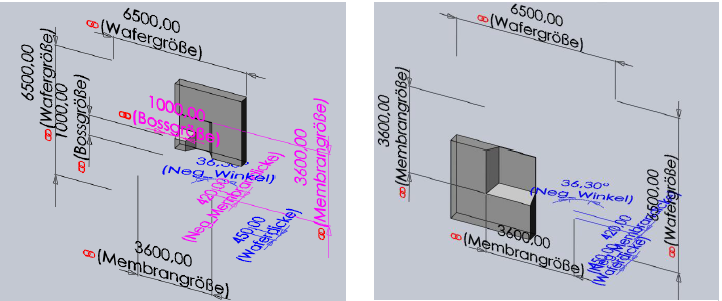
\includegraphics[width=0.9\textwidth]{figures/viertel.png}
	\caption{Gevierteltes CAD-Modell ohne Boss (links), mit Boss (rechts)}
	\label{fig:viertel}
\end{figure}
\section{FEM-Simulation (Justus)}
\label{sec:FEM}
Nachdem die CAD-Modelle erstellt sind, wird eine FEM-Simulation der geviertelten Modelle durchgef�hrt. Dazu wird der Wafer an den Schnittkanten, au�er an der Membran, fest eingespannt. Dies kann einfach in SolidWorks eingestellt werden. Weitere Vorgaben sind
\begin{itemize}
\item die Elemtentgr��e auf der Membran von 60$\mu$m
\item eine globale Elemtentgr��e von 120$\mu$m
\item vorgegebener Druck von 1bar
\end{itemize}
sowie die in Tabelle \ref{tab:materialeig} dargestellten Materialeigenschaften f�r Silizium, die in die Materialdatenbank von SolidWorks eingepflegt werden k�nnen. 
\begin{table}[h]
\centering
\caption{Materialeigenschaften Silizium}
\label{tab:materialeig}
\begin{tabular}{|c|c|}
\hline
Elastizit�tsmodul (E) & 169GPa      \\ \hline
Poissonzahl ($\nu$)        & 0,279     \\ \hline
Schubmodul (G)        & 50,85GPa \\ \hline
Dichte ($\rho$)             &  \SI{2,33}{\gram\per\cubic\centi\meter}     \\ \hline
Bruchspannung ($\sigma$)      & 380MPa   \\ \hline
\end{tabular}
\end{table}

\subsection{Ermittlung der Spannungsverl�ufe (Justus)}
\label{subsec:ermittlung der spannungsverl�ufe}
Durch eine erste Simulation sollen die Spannungsverl�ufe entlang der Schnittkanten bestimmt werden. Dazu wird f�r beide Designs die Standardabmessung verwendet. Abbildung \ref{pl:ohneBoss} und Abbildung \ref{pl:mitBoss} illustrieren die Spannungsverl�ufe $\sigma_z$ und $\sigma_x$ �ber den Weg x, also den Abstand zum Sensorrand, f�r das Design ohne und mit Boss. Das Ergebnis ist ist ebenfalls in Abbildung \ref{fig:visualisierung} zu erkennen, die die Spannung am Bauteil selbst visualisiert.
\begin{figure}[H]
	\centering
	\begin{tikzpicture}\centering
	\begin{axis}[,xlabel={x / $\mu$m},ylabel={$\sigma$ / Pa},legend pos=north east,legend columns=1,xtick distance=500]
	\pgfplotstableread{chapters/Daten/ohneBossStat.dat}\data
	
	\addplot [color1] table [x=X,y=sigma] {\data};
	
	\end{axis}
	\end{tikzpicture}
	\caption{Spannungsverlauf einer Membran ohne Boss bei \unit[1]{bar}/strain curve of a membrane without boss at \unit[1]{bar}}\label{pl:ohneBoss}
%	\vspace{10mm}
	\centering
	\begin{tikzpicture}\centering
	\begin{axis}[,xlabel={x / $\mu$m},ylabel={$\sigma$ / Pa},legend pos=north east,legend columns=1,xtick distance=500]
	\pgfplotstableread{chapters/Daten/mitBossStat.dat}\data
	
	\addplot [color1] table [x=X,y=sigma] {\data};
	\addlegendentry{$\sigma_x$}
	
	\pgfplotstableread{chapters/Daten/mitBossStat2.dat}\data
	
	\addplot [color2] table [x=z,y=sigma] {\data};
	\addlegendentry{$\sigma_z$}
	
	\end{axis}
	\end{tikzpicture}
	\caption{Spannungsverlauf einer Membran mit Boss bei \unit[1]{bar}/ strain curve of a membrane with boss at \unit[1]{bar}}\label{pl:mitBoss}
\end{figure}
\begin{figure}[H]
	\centering
  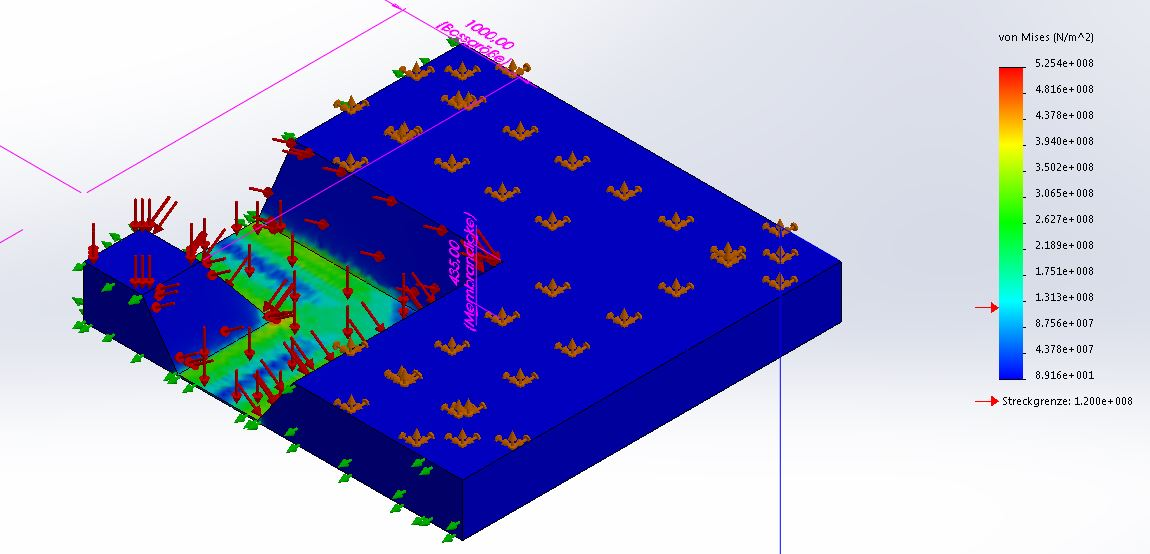
\includegraphics[width=0.7\textwidth]{figures/10-2_Spannung.JPG}
	\caption{Visualisierung der FEM-Simulation am Bauteil}
	\label{fig:visualisierung}
\end{figure}
Da sich die Spannungsverl�ufe f�r das Design ohne Boss sehr �hneln, wird lediglich einer der beiden ermittelten im Diagramm aufgetragen. \\
Beim Vergleich der Verl�ufe ist zu erkennen, dass die jeweilige Maximalspannungen jeweils am �bergang von der Schr�gen zur Membran auftreten. Das bedeutet, dass dort am ehesten ein Versagen zu erwarten ist. Dem kann entgegengewirkt werden, indem entsprechende Bereiche verst�rkt werden. Beispielsweise k�nnte im Herstellungsprozess, also beim �tzen, eine geeignete Kompensationsstruktur verwendet werden, um einen besseren �bergang zwischen Schr�ge und Membran zu erzielen. \\
Weiterhin ist anzumerken, dass die Maximalspannung f�r den Sensor ohne Boss leicht gr��er ist als jene f�r das Design mit Boss. Dar�ber hinaus ist die Spannung bei dem Design mit Boss besser verteilt, die Belastungen verteilen sich also auf verschiedene Bereiche des Sensors. Durch den Boss wird eine �hnlich hohe Maximalspannung wie beim Design ohne Boss verhindert. Wie in Abbildung \ref{pl:mitBoss} zu erkennen ist, schrumpft die Spannung im Bereich der Bossstruktur auf ein Minimum. \\
Weiterhin ist zu beobachten, dass $\sigma_x$ f�r die Struktur mit Boss deutlich h�here Werte aufweist als $\sigma_z$. Au�erdem ist $\sigma_z$ gestauchter als $\sigma_x$. \\
%\\
%\begin{figure}[h]
%	\centering
%	\begin{tikzpicture}\centering
%	\begin{axis}[,xlabel={x / $\mu$m},ylabel={$\sigma$ / Pa},legend pos=north east,legend columns=1,xtick distance=500]
%	\pgfplotstableread{chapters/Daten/mitBossStat.dat}\data
%	
%	\addplot [color1] table [x=X,y=sigma] {\data};
%	\addlegendentry{$\sigma_x$}
%	
%	\pgfplotstableread{chapters/Daten/mitBossStat2.dat}\data
%	
%	\addplot [color2] table [x=z,y=sigma] {\data};
%	\addlegendentry{$\sigma_z$}
%	
%	\end{axis}
%	\end{tikzpicture}
%	\caption{Spannungsverlauf einer Membran mit Boss bei \unit[1]{bar}/ strain curve of a membrane with boss at \unit[1]{bar}}\label{pl:mitBoss}
%\end{figure}


\subsection{Einfluss der Membrandicke auf die maximale Spannung (Viviane Bremer)}
\label{subsec:Membrandicke}

In diesem Abschnitt wird der Einfluss der Membrandicke auf die auftretende mechanische Spannung in der Membran betrachtet. Hierf�r werden folgende Dicken genutzt: \unit[15]{$\mu$m}, \unit[25]{$\mu$m}, ,\unit[35]{$\mu$m}.

%\begin{itemize}
%	\item[a.] \unit[15]{$\mu m$}
%	\item[b.] \unit[25]{$\mu m$}
%	\item[c.] \unit[35]{$\mu m$}	
%\end{itemize}

Zur Analyse wird der anliegende Druck f�r alle drei Membrandicken in \unit[0.2]{bar}-Schritten von \unit[0.2]{bar} bis \unit[1]{bar} erh�ht und die resultierende mechanische Spannung ermittelt. Die Verl�ufe sind in Abbildung \ref{pl:Membrandicken} dargestellt. Die Bruchspannung $\sigma_{Br}$ von Silizium betr�gt \unit[830]{MPa} und sollte w�hrend des Sensorbetriebs nicht �berschritten werden. Zur besseren Visualisierung ist sie als Konstante im Graphen dargestellt.

\begin{figure}[H]
	\centering
	\begin{tikzpicture}\centering
	\begin{axis}[width=0.8\textwidth, xlabel={p / bar},ylabel={$\sigma$ / Pa},legend pos=north west,legend columns=1,xtick distance=0.2]
	\pgfplotstableread{chapters/Daten/Membran.dat}\data

	\addplot [red] table [x=p415,y=bruch415] {\data};
	\addlegendentry{$\sigma_{Br}$}
	
	\addplot [color1] table [x=p415, y=sigx415] {\data};
	\addlegendentry{$\sigma_x$: \unit[35]{$\mu$m}}
	
	\addplot [color2] table [x=p415,y=sigz415] {\data};
	\addlegendentry{$\sigma_z$: \unit[35]{$\mu$m}}
	
	\addplot [color4] table [x=p415,y=sigx425] {\data};
	\addlegendentry{$\sigma_x$: \unit[25]{$\mu$m}}

	\addplot [color3] table [x=p415,y=sigz425] {\data};
	\addlegendentry{$\sigma_z$: \unit[25]{$\mu$m}}
	
	\addplot [blue] table [x=p415,y=sigx435] {\data};
	\addlegendentry{$\sigma_x$: \unit[15]{$\mu$m}}
	
	\addplot [yellow] table [x=p415,y=sigz435] {\data};
	\addlegendentry{$\sigma_z$: \unit[15]{$\mu$m}}
	
	\end{axis}
	\end{tikzpicture}
	\caption{Spannungsverlauf der drei Membrandicken}\label{pl:Membrandicken}
\end{figure}

Membran a erreicht die Bruchspannung schon bei einem Druck von \unit[0.439]{bar}, welcher im ben�tigten Messbereich liegt. Im Falle von Membran b wird sie knapp oberhalb des Messbereichs bei \unit[1.05]{bar} erreicht. Die Bruchspannung bei Membran c entspricht einem anliegenden Druck von \unit[2]{bar}, welcher deutlich oberhalb des Messbereiches ist. Hieraus lassen sich Erkenntnisse f�r das Sensorverhalten gewinnen. Membran a ist zu d�nn f�r diese Messaufgabe, da sie innerhalb des Messbereichs rei�t. Jedoch ist Membran c auch nicht akzeptabel, da durch die gr��ere Membrandicke niedrigere Spannungen auftreten im Vergleich zu Membran b. Diese bildet einen guten Kompromiss f�r die gew�nschte Aufgabe.


\subsection{Einfluss der Membranabmessungen auf den Spannungsverlauf}
\label{subsec:Membranabmessungen}

\begin{figure}[H]
	\centering
	\begin{tikzpicture}\centering
	\begin{axis}[,xlabel={x / $\mu$m},ylabel={$\sigma$ / Pa},legend pos=north east,legend columns=1,xtick distance=500]
	\pgfplotstableread{chapters/Daten/Membran3200.dat}\data
	
	\addplot [color1] table [x=X,y=Wert] {\data};
	\addlegendentry{$\sigma$: \unit[3200]{$\mu$m}}
	
	\pgfplotstableread{chapters/Daten/Membran4000.dat}\data
	
	\addplot [color2] table [x=Y,y=Wert] {\data};
	\addlegendentry{$\sigma$: \unit[4000]{$\mu$m}}
	
	
	\end{axis}
	\end{tikzpicture}
	\caption{Spannungsverlauf der Membrangr��en}\label{pl:Membranesize}
\end{figure}

\subsection{Einfluss der Bossgr��e (Viviane Bremer)}
\label{subsec:Bosssize}

Zur Analyse des Einflusses der Bossgr��e wird die Membrangr��e auf \unit[3600]{$\mu$m} und die Membrandicke auf \unit[25]{$\mu$m} gesetzt. Die Bossgr��e wird folgenderma�en variiert: \unit[800]{$\mu$m}, \unit[1000]{$\mu$m}, \unit[1200]{$\mu$m}.

Die Spannungsverl�ufe und Verschiebungen sind in Abbildung \ref{pl:Bosssize} dargestellt. Bei einer Bossgr��e von \unit[800]{$\mu$m} treten Spannungen von bis zu \unit[274]{MPa} auf. Eine Vergr��erung des Bosses auf \unit[1000]{$\mu$m} f�hrt zu einer maximalen Spannung von  \unit[178]{MPa}. Der gr��te Boss senkt die auftretende Spannung auf \unit[128]{MPa}. Des Weiteren ist zu sehen, dass eine Vergr��erung des Bosses zu einer Angleichung der Spannungsspitzen f�hrt und die Dehnung der Membran von \unit[374]{$\mu$m} auf \unit[77]{$\mu$m} senkt.

\begin{figure}[H]
	\centering
	\begin{tikzpicture}\centering
	\begin{axis}[,xlabel={x / $\mu$m},ylabel={$\sigma$ / Pa},legend pos=north east,legend columns=1,xtick distance=500]
	\pgfplotstableread{chapters/Daten/MechSpannung.dat}\data
	
	\addplot [color1] table [x=X1,y=sigma1] {\data};
	\addlegendentry{$\sigma$: \unit[800]{$\mu$m}}
	
	\addplot [color2] table [x=X2,y=sigma2] {\data};
	\addlegendentry{$\sigma$: \unit[1000]{$\mu$m}}
	
	\addplot [color3] table [x=X3,y=sigma3] {\data};
	\addlegendentry{$\sigma$: \unit[1200]{$\mu$m}}
	
	\end{axis}
	\end{tikzpicture}
	\caption{Spannungsverlauf der drei Bossgr��en}\label{pl:Bosssize}
\end{figure}
\subsection{Platzierung der Widerst�nde der Messbr�cken (Justus)}
\label{platzierung}
Bei Messungen mit Messbr�cken nach Wheatstone wird der piezoresistive Effekt ausgenutzt. Durch eine Dehnung bzw. Stauchung der verwendeten Resistoren wird eine Widerstands�nderung erzeugt, die die Messspannung beeinflusst. Um diesen Effekt voll ausnutzen zu k�nnen, liegt es nahe, die Widerst�nde in dem Bereich anzubringen, wo die gr��te Dehnung vorliegt. Durch die FEM-Simulation wurde gezeigt, dass dies an den �berg�ngen von Membran zu Waferstruktur bzw. zum Boss der Fall ist. Deshalb sollten die Br�ckenwiderst�nde auch in diesen Bereichen platziert werden.
\subsection{Kritische Betrachtung (Justus)}
\label{kritische betrachtung}
Eine FEM-Simulation wird meistens unter idealen Bedingungen durchgef�hrt, da sich in der Realit�t auftretende St�reinfl�sse schlecht simulieren lassen. Zun�chst gibt es, gerade bei Mikrosystemen, welche im h�ufigsten Fall durch �tzen hergestellt werden, stets Fertigungstoleranzen. Diese beeinflussen nicht die Simulation, aber �ndern das Verhalten des realen Bauteils. Hinzu kommt, dass das Silizium, das f�r die Simulation verwendet wurde, als isotroper Werkstoff simuliert wird. Dies bedeutet, dass das Materialverhalten in alle Raumrichtungen gleich ist. In der Realit�t ist Silizium jedoch, unter anderem bedingt durch seine monokristalline Struktur, anisotrop. Anisotropie bedeutet die Richtungsabh�ngigkeit des Materialverhaltens, die den Rechenaufwand einer Simulation enorm vergr��ern w�rde. Ein Beispiel f�r die Verwendung von Anisotropie in Bezug auf Silizium ist die Ber�cksichtigung der Miller'schen Indizes beim �tzprozess. Als weiterer Grund f�r eine Abweichung der FEM-Simulation zur Realit�t ist die gew�hlte Elementgr��e von 60 bzw. 120 $\mu$m. Es besteht zwar die M�glichkeit, die Vorgaben weiter zu verfeinern, jedoch bleiben steht Bereiche, auf denen interpoliert werden muss. Au�erdem vergr��ert sich bei genaueren Analysen die Rechenzeit enorm.\\
Abschlie�end kann behauptet werden, die durchgef�hrten Simulationen sind lediglich eine grobe Ann�herung an das reale Systemverhalten.

\section{Zusammenfassung (Manish)}
\label{sec:zusammenfassung2}

\chapter{Etching Process}
\label{sec:EtchingProcess}


\section{Der Reaktionsprozess beim Silizium�tzen (Viviane)}
F�r die Erstellung der Sensormembran muss zun�chst der �tzprozess mit KOH charakterisiert werden. Die Reaktion besteht aus der Oxidation und einer Reduktion des Siliziums. Somit ergibt sich die Reaktionsgleichung zu

\begin{equation}
	Si + 2OH^- + 2H_2O \longrightarrow SiO_2(OH)_2^{2-} + 2H_2. \label{eq:reaction}
\end{equation}

Zur Berechnung des zu �tzenden Volumens der Membran wird folgende Volumenformel eines Pyramidenstumpfes, 

\begin{equation}
	V = \frac{h}{3}(A_1 + \sqrt{A_1 A_2} + A_2), \label{eq:Pyramide}
\end{equation}
 

ben�tigt. F�r die Fertigung wird ein 4''-Wafer mit einer Dicke von \unit[450]{$\mu$m} genutzt. Die zu erzeugende Membran ohne Boss hat eine Breite von \unit[4000]{$\mu$m} und eine Dicke von \unit[25]{$\mu$m}. Dies f�hrt zu einer �tzh�he von

\begin{equation}
	h = 450\,\mu m - 25\,\mu m = 425\,\mu m.
\end{equation}

Die Fl�che $A_1$ bestimmt sich mit der Membranbreite zu

\begin{equation}
	A_1 = a_1^2 = 4000\,\mu m \cdot 4000\,\mu m = 16\,mm^2.
\end{equation}

Fl�che $A_2$ ergibt sich mit

\begin{align}
	\tan(54,7�) &= \frac{425\,\mu m}{\Delta a} \\
	\Delta a &= \frac{425\,\mu m}{\tan(54,7�)} = 300\,\mu m\\
	a_2 &= a_1 - 2 \Delta a = 3400\,\mu m
\end{align}

zu

\begin{equation}
	A_2 = a_2^2 = 11,56\,mm^2.
\end{equation}

Dies eingesetzt in Gleichung \ref{eq:Pyramide} ergibt f�r das zu �tzende Volumen

\begin{equation}
	V_{Si} = \frac{0.425\,mm}{3}(16 + \sqrt{16 \cdot 11.56} +11.56)\,mm^2 = 5.831\,mm^3.
\end{equation}

Die Dichte $\rho_{Si}$ von Silizium betr�gt \unitfrac[0.002336]{g}{$mm^3$}. Dies f�hrt mit dem errechneten Volumen zu einer Masse von

\begin{equation}
	m_{Si} = \rho V_{Si} = 0.0137\,g
\end{equation}

Mit der Molmasse von Silizium, $M_{Si} = $\unitfrac[28.09]{g}{mol}, ergibt sich die Stoffmenge zu

\begin{equation}
	n_{Si} = \frac{m_{Si}}{M_{Si}} = 4.877 \cdot 10^{-4} mol.
\end{equation}

Wie in Gleichung \ref{eq:reaction} zu sehen, entstehen bei der Reaktion zwei Teile Wasserstoff. Somit ergibt sich f�r die Stoffmenge des Wasserstoffs

\begin{equation}
	n_{H_2} = 2n_{Si} = 2 \cdot 4.877 \cdot 10^{-4}\,mol = 9.754 \cdot 10^{-4}\,mol.
\end{equation}

Damit kann das Volumen mit dem molaren Normvolumen des idealen Gases $V_{m,0}=\unitfrac[22.414]{l}{mol}$ zu

\begin{equation}
	V_{H_2} = V_{m,0} \cdot n_{H_2} = 22.414\,\unitfrac{l}{mol} \cdot 9.754 \cdot 10^{-4}\,mol = 0.0218\,l
\end{equation}

bestimmt werden. Da dies ein sehr geringes Volumen ist, reicht eine gute Bel�ftung als Vorsichtsma�nahme aus. Eine weitere Ma�nahme w�re noch die Beseitigung von Z�ndquellen.

Bei dem �tzprozess werden des Weiteren zwei Teile Wasser umgesetzt. Das Volumen entspricht somit

\begin{align}
	n_{H_2O} &= n_{H_2} = 9.754 \cdot 10^{-4}\,mol \\
	m_{H_2O} &= M_{H_2O} \cdot n_{H_2O} = \unitfrac[18]{g}{mol} \cdot 9.754 \cdot 10^{-4}\,mol = 0.0175\,g\\
	V_{H_2O} &= \dfrac{m_{H_2O}}{\rho_{H_2O}} = \dfrac{0.0175\,g}{1 \unitfrac{g}{cm^3}} = 0.0175\,cm^3 = 0.0175\,ml.
\end{align}

Der �tzprozess soll mit einer 40\%-ige KOH-L�sung auf Basis von zwei Litern Wasser durchgef�hrt werden. Das bedeutet, dass

\begin{equation}
	m_{KOH} = 0.4 m_{H_2O} = 0.4 \cdot \unit[2]{kg} = \unit[800]{g}
\end{equation}

KOH-Salz ben�tigt wird. Dies entspricht einer Stoffmenge von

\begin{equation}
	n_{KOH} = \dfrac{m_{KOH}}{M_{KOH}} = \dfrac{\unit[800]{g}}{\unitfrac[56.11]{g}{mol}} = \unit[14.258]{mol}.
\end{equation}

\section{Weitere Anmerkungen (Justus)}
\label{�tzen2}
Aus der Reaktionsgleichung zum Silizium�tzen (vgl. Gleichung \ref{eq:reaction}) geht hervor, dass die Konzentration der KOH-L�sung w�hrend des �tzprozesses nicht ver�ndert wird. Dies ist daran zu erkennen, dass auf beiden Seiten der Gleichung die selbe Menge Wasserstoff vorhanden ist, folglich geht kein Wasserstoff verloren. Anders w�re dies, wenn mehr Wasser bzw. Wasserstoff verbraucht werden w�rde, als als Reaktionsergebnis herauskommt. Dies w�rde bedeuten, dass beim �tzprozess Wasserstoff verbraucht wird, wodurch sich die Konzentration der KOH-L�sung erh�hen w�rde. Prozesse, wodurch sich die Konzentration erh�hen w�rde, sind beispielsweise Verdunstung oder die Reaktion mit $CO_2$. \\
Weiterhin sollte beim �tzprozess die genaue Rotationsverschiebung von Maske und Wafer genau bekannt sein, um Unter�tzungen zu vermeiden.\\
Ein wichtiger Faktor ist die �tzrate, die durch 
\begin{equation}
r = \dfrac{�tztiefe}{�tzzeit} = \dfrac{\Delta{z}}{\Delta{t}}
\end{equation}
definiert ist. Damit lassen sich die voraussichtlichen �tzzeiten f�r die Membrandicken 15, 25, und 35$\mu$m berechnen.
Mit \begin{equation}
\Delta{t} = \dfrac{\Delta{z}}{r}
\end{equation}
ergeben sich f�r mit einer �tzrate f�r die Raumrichtung <110> von $100,6 \dfrac{\mu{m}}{h}$ die folgenden �tzzeiten (vgl. Tabelle \ref{tab:�tzzeit}).
\begin{table}[h]
\centering
\caption{�tzzeiten f�r verschiedene Membrandicken}
\label{tab:�tzzeit}
\begin{tabular}{|c|c|}
\hline
\textbf{Membrandicke {[\textbf{$\mu$}m}{]}} & \textbf{�tzzeit {[}h{]}} \\ \hline
15                           &   4,324                       \\ \hline
25                           &      4,22                    \\ \hline
35                           &          4,125                \\ \hline
\end{tabular}
\end{table}

\chapter{Characterising}
\label{sec:Characterising}



\section{Allgemeines (Justus)}
\label{sec:Unit}
Nachdem am ersten Labortag der Sensor mit Hilfe von SolidWorks designt und auf theoretischer Grundlage mit verschiedenen Simulationen berechnet wurde, soll nun eine Charakterisierung erfolgen. Aufgrund von Fertigungsabweichungen, die nie vermieden werden k�nnen, verhalten sich Sensoren immer unterschiedlich. Dies spiegelt sich unter Anderem in der Sensitivit�t, dem Offset oder auch in der Messgenauigkeit wider. Um den Abweichungen entgegenzuwirken, m�ssen bestimmte Eigenschaften des entsprechenden Sensors also zun�chst ermittelt werden.
Am IMT ist eine Reihe von Sensoren verf�gbar, die sich mit blo�em Auge nicht unterscheiden lassen. Lediglich bei der Betrachtung unter dem Mikroskop lassen sich Differenzen feststellen. Der Unterschied zwischen den Drucksensoren ergibt sich aus der Anordnung der jeweiligen Resistoren, die stellenweise in die Sensormembran eingearbeitet sind und der piezoresistiven Spannungsmessung dienen.
%INCLUDE SENSORBILDER UNTER MIKROSKOP
Abbildung \ref{fig:Sensordesign} a) zeigt eine t-f�rmige Anordnung der Resistoren, Abbildung \ref{fig:Sensordesign} b) eine transversale. Eine Festlegung, welche Anordnung f�r die gegebenen Anforderungen am besten geeignet sei, erschlie�t sich aus �berlegungen. %WARUM ??
\\
\begin{figure}[h]
    \subfigure[Messbr�cke mit t-f�rmiger Anordnung]{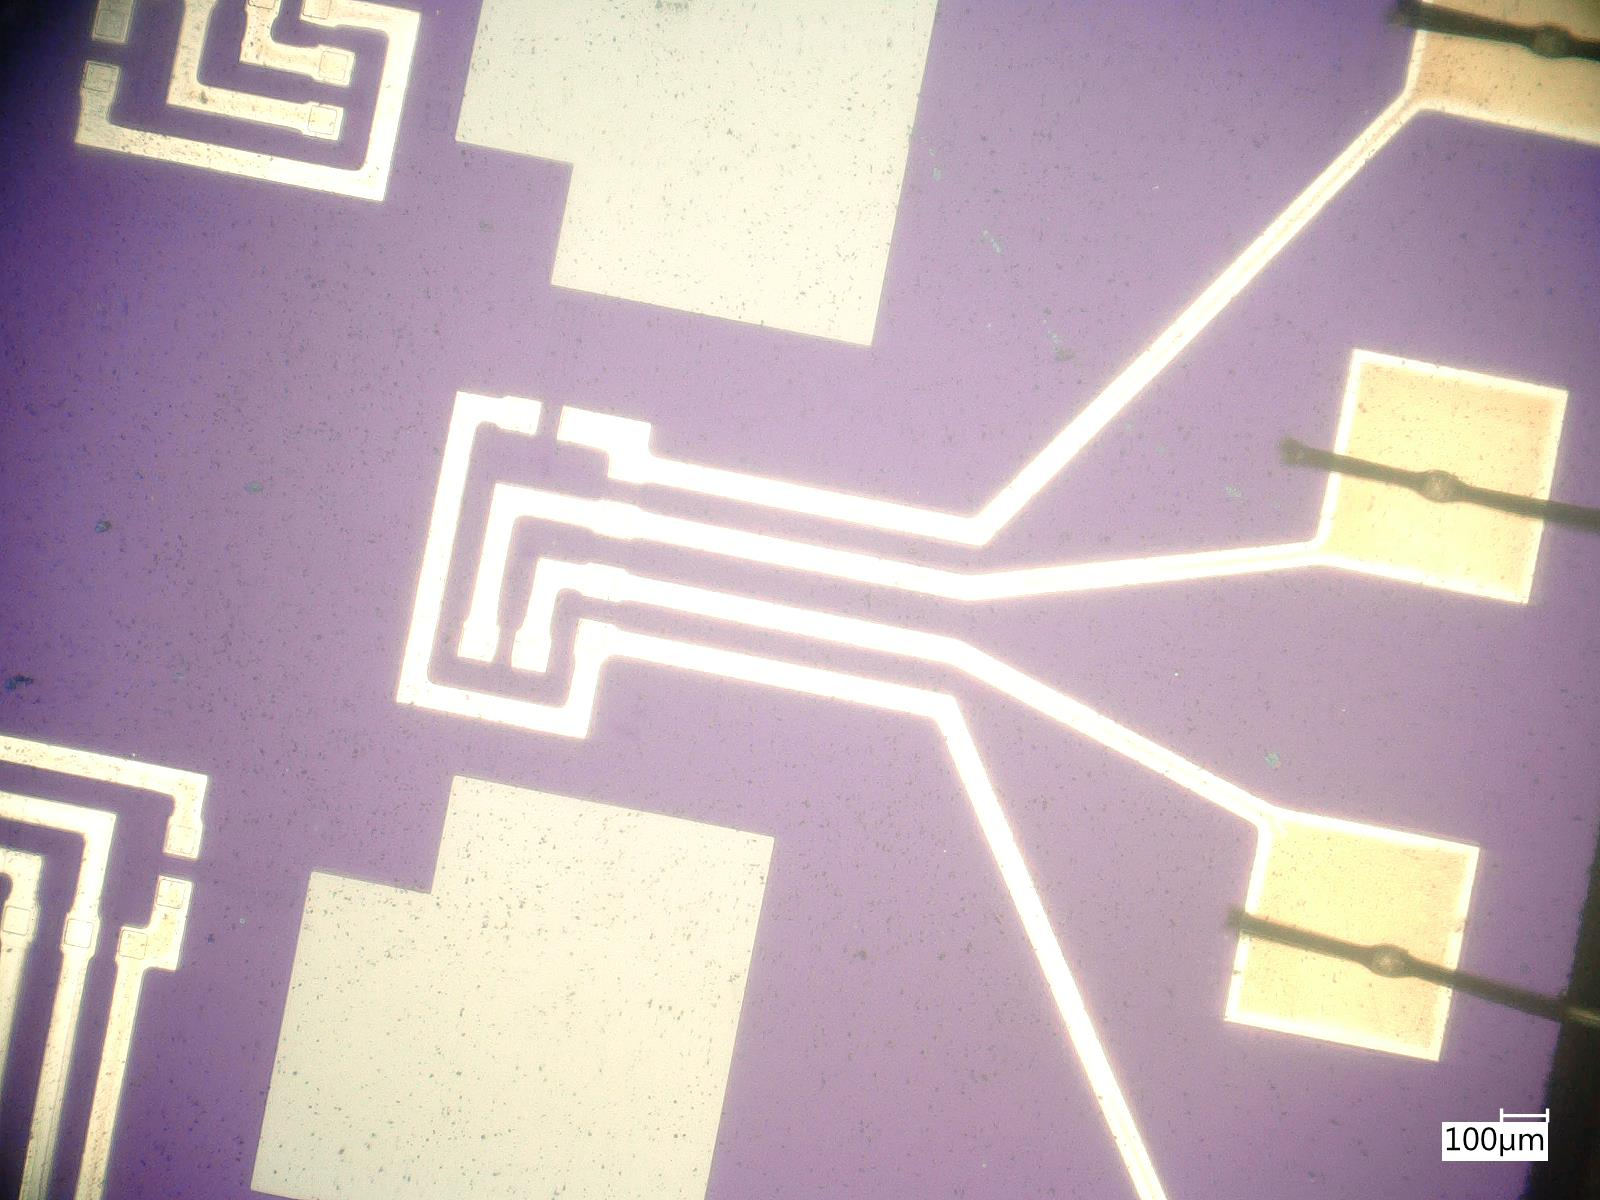
\includegraphics[width=0.49\textwidth]{figures/microscope_sensor/M_11_sensor.jpg}} 
    \subfigure[Messbr�cke mit transversaler Anordnung]{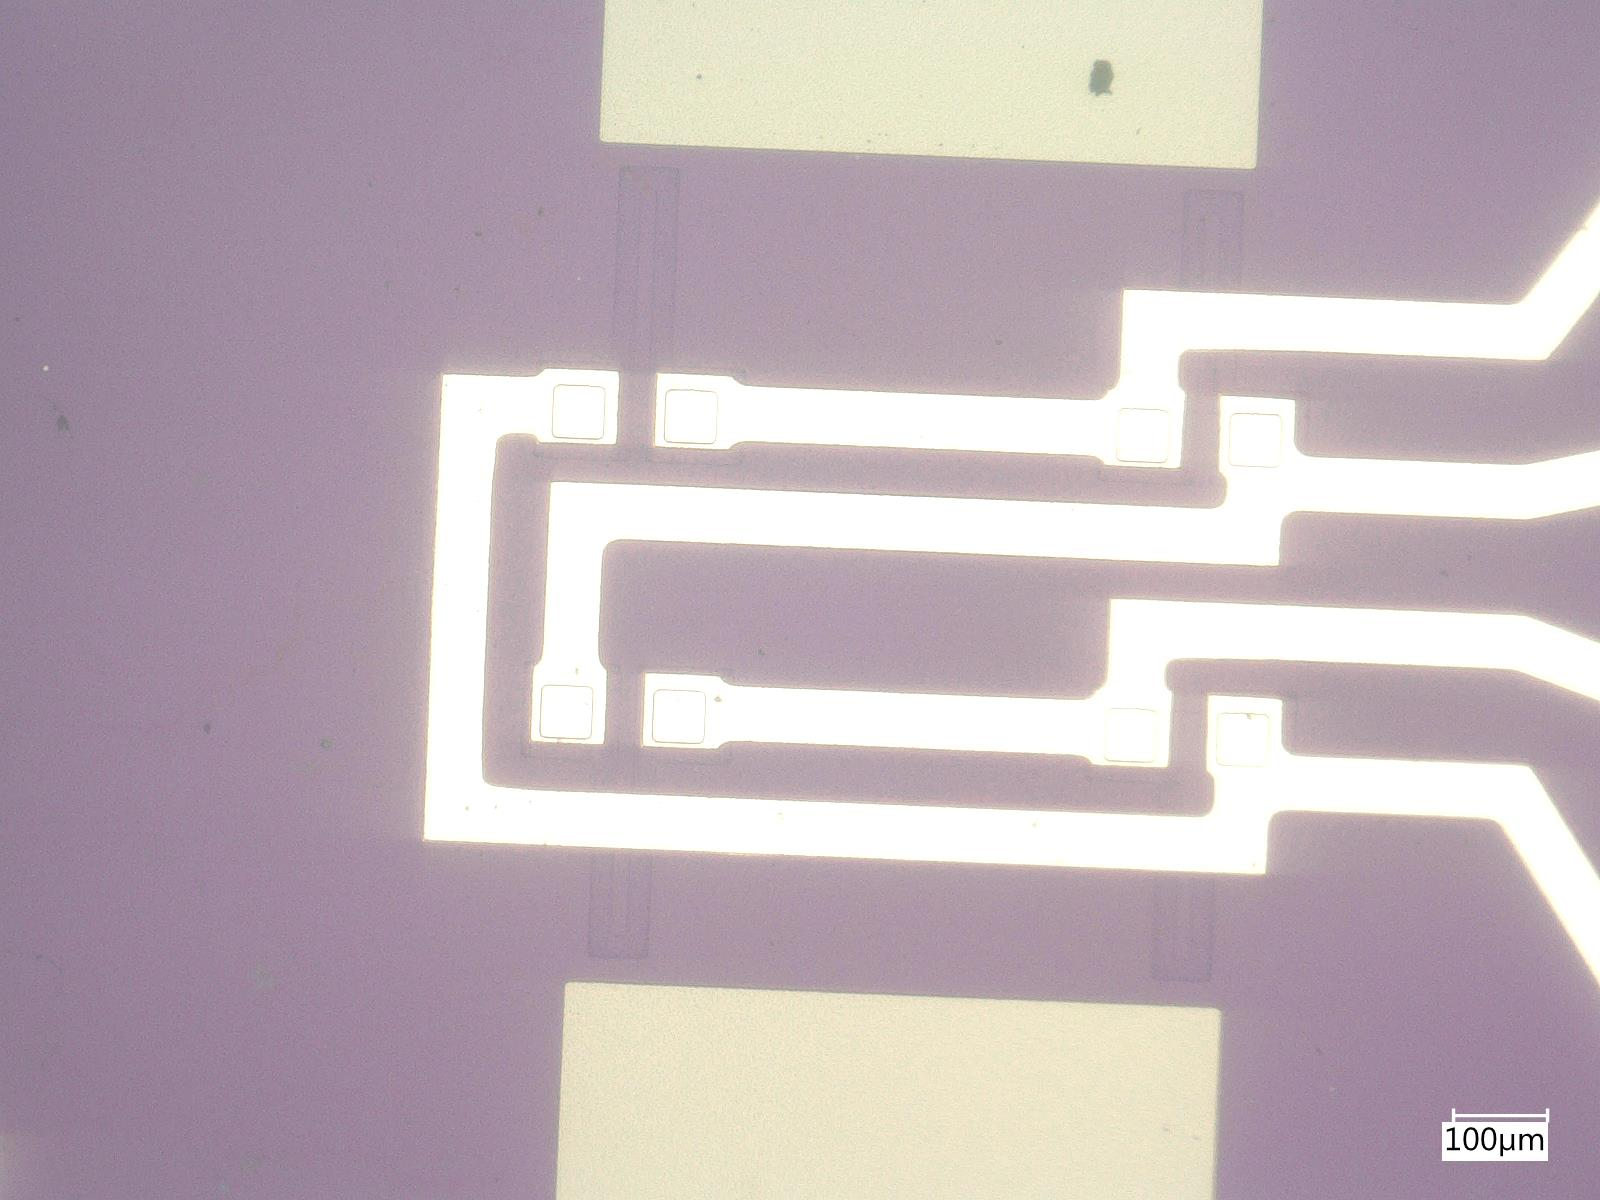
\includegraphics[width=0.49\textwidth]{figures/microscope_sensor/Justus_Sensor-13_200.jpg}}
\caption{Sensordesigns im �berblick}\label{fig:Sensordesign}
\end{figure}\\

Anschlie�end begann die eigentliche Charakterisierung in Form eines Versuchs.
%Viele Einheiten lassen sich sch�ner darstellen mit dem "`Tag"' \verb|\unit[]{}| beziehungsweise \verb|\unitfrac[]{}{}|. Siehe den Vergleich: ohne 1~m oder mit \unit[1]{m} bzw. ohne 1~m/sec oder mit \unitfrac[1]{m}{sec}.

\section{Versuchsaufbau und -durchf�hrung (Justus)}
\label{sec:Quelltext}
Der jeweilige Sensor wird auf eine Steckplatine mit entsprechenden Ein- und Ausg�ngen gesetzt. Die Versorgungsspannung von 1V wird durch eine externe Spannungsquelle bewerkstelligt. Zur Messung der Ausgangsspannung steht ein Multimeter zur Verf�gung, das ebenfalls mit der Steckplatine verbunden wird. Bevor die Verbindungen angebracht werden, m�ssen zun�chst die Leiterbahnen der Platine betrachtet werden, um Ein- und Ausg�nge nicht zu verwechseln. Der Druck wird mit Hilfe eines Druckreglers aufgegeben, welcher den Gasdruck von Stickstoff exakt aufbringen kann. Abbildung \ref{fig:singlepicture} zeigt den gesamten Versuchsaufbau.

\begin{figure}[h]
  \centering
  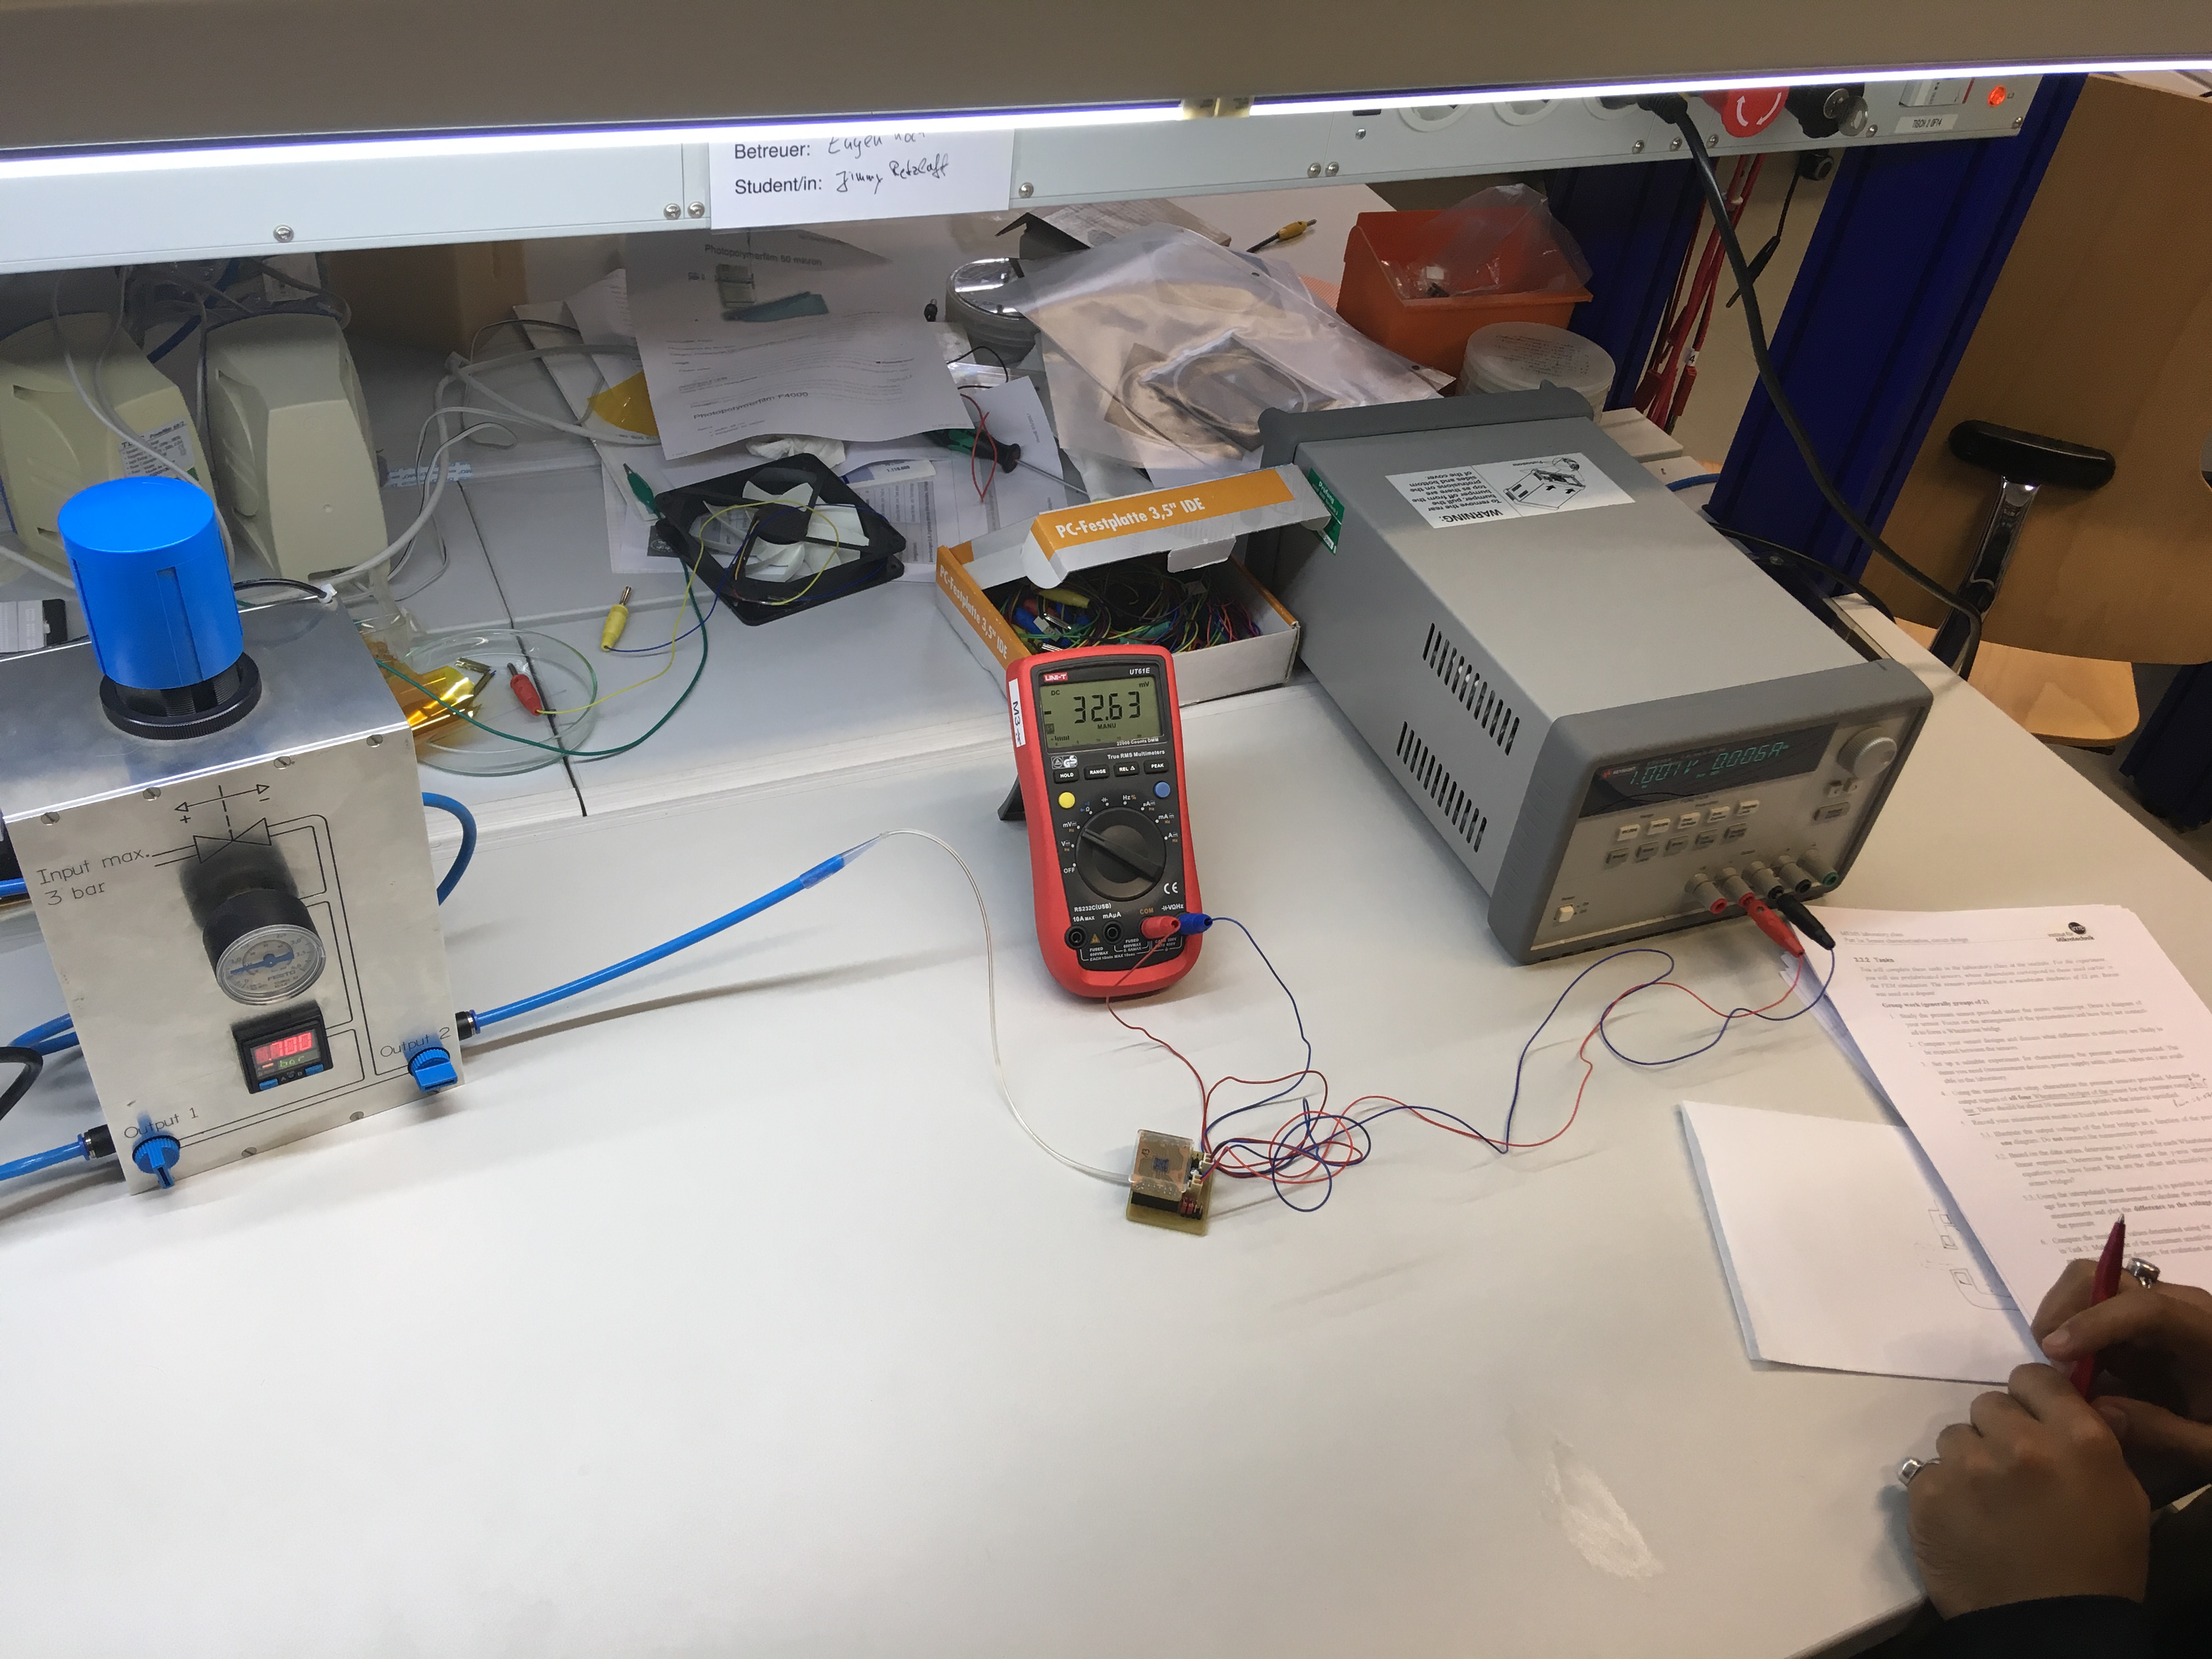
\includegraphics[width=0.7\textwidth]{figures/Versuchsaufbau1.jpg}
  \caption{Versuchsaufbau zur Charakterisierung}
  \label{fig:singlepicture}
\end{figure}

Da jede der vier zum Sensor geh�renden Wheatstone'schen Messbr�cken charakterisiert werden muss, werden entsprechende Jumper verwendet, mit denen die einzelnen Messbr�cken angesteuert werden k�nnen. Zu jeder Br�cke wird die Ausgangsspannung f�r die Dr�cke 0bar, 0,2bar, 0,4bar, 0,6bar, 0,8bar und 1bar gemessen und festgehalten. Au�erdem ist es sinnvoll, je eine Messung ohne Anschluss an die Druckversorgung durchzuf�hren, um einen Messwert unter atmosph�rischem Druck zu erhalten. 


\section{Auswertung (Viviane)}
\label{sec:Auswertung}

Die Messergebnisse der zwei Sensoren sind in Abbildung \ref{pl:Messwerte} dargestellt. Anhand der Graphen ist deutlich zu erkennen, dass eine t-f�rmige Anordnung f�r diese Anwendung nicht zielf�hrend ist. Die ermittelten Kennlinien f�r die einzelnen Br�cken dieses Designs sind nahezu konstant. Im Gegensatz dazu zeigen die Kennlinien des transversalen Designs einen deutlich linear steigenden Verlauf. Bei diesem Sensor wurde die Messwerte der Br�cke 3 f�r den Umgebungsdruck und f�r \unit[0.08]{bar} herausgenommen, da diese einen deutlich gr��eren Wert vorweisen als der f�r \unit[0.1]{bar}, was einem unphysikalischen Verhalten entsprechen w�rde.

% Jedoch weicht der errechnete Wert bei der t-f�rmigen Anordnung nicht so stark vom gemessenen Wert ab, wie bei dem transversalen Design (Abbildung \ref{pl:Abweichung}).

\begin{figure}[htb]
	\centering
	\begin{tikzpicture}[trim axis left]
	\begin{groupplot}[
	group style={columns=1, rows=2, vertical sep=10pt, x descriptions at=edge bottom,},
	width = 0.7 \textwidth, 
	xlabel={p / bar},ylabel={U / mV},legend pos=south east,legend columns=2,
	]
	
	\nextgroupplot[ylabel={U / mV},title=t-f�rmiger Sensor, height=7cm,]
	\pgfplotstableread{chapters/Daten/Sensor_11.dat}\data
	
	\addplot [only marks,color1,mark=x] table [x=p1,y=V1] {\data};
	\addplot [mark=none, color1] table [x=p1,y={create col/linear regression={y=V1}}] {\data};
	\xdef\Slopea{\pgfplotstableregressiona}
	\xdef\Offseta{\pgfplotstableregressionb}
	\addlegendentry{B1}
	\addlegendentry{$f_{\text{Reg,B1}}=\pgfmathprintnumber{\Slopea}x\pgfmathprintnumber[print sign]{\Offseta}$}
	
	\addplot [only marks,color2] table [x=p2,y=V2] {\data};
	\addplot [mark=none, color2] table [x=p2,y={create col/linear regression={y=V2}}] {\data};
	\xdef\Slopeb{\pgfplotstableregressiona}
	\xdef\Offsetb{\pgfplotstableregressionb}
	\addlegendentry{B2}
	\addlegendentry{$f_{\text{Reg,B2}}=\pgfmathprintnumber{\Slopeb}x\pgfmathprintnumber[print sign]{\Offsetb}$}
	
	\addplot [only marks,color3] table [x=p3,y=V3] {\data};
	\addplot [mark=none, color3] table [x=p3,y={create col/linear regression={y=V3}}] {\data};
	\xdef\Slopec{\pgfplotstableregressiona}
	\xdef\Offsetc{\pgfplotstableregressionb}
	\addlegendentry{B3}
	\addlegendentry{$f_{\text{Reg,B3}}=\pgfmathprintnumber{\Slopec}x\pgfmathprintnumber[print sign]{\Offsetc}$}
	
	\addplot [only marks,color4] table [x=p4,y=V4] {\data};
	\addplot [mark=none, color4] table [x=p4,y={create col/linear regression={y=V4}}] {\data};
	\xdef\Sloped{\pgfplotstableregressiona}
	\xdef\Offsetd{\pgfplotstableregressionb}
	\addlegendentry{B4}
	\addlegendentry{$f_{\text{Reg,B4}}=\pgfmathprintnumber{\Sloped}x\pgfmathprintnumber[print sign]{\Offsetd}$}
	
	
	
	\nextgroupplot[xlabel={p / bar}, ylabel={U / mV},title=transversaler Sensor, height=7cm,]
	\pgfplotstableread{chapters/Daten/Sensor_13.dat}\data
	
	\addplot [only marks,color1,mark=x] table [x=p1,y=V1] {\data};
	\addplot [mark=none, color1] table [x=p1,y={create col/linear regression={y=V1}}] {\data};
	\xdef\Slopea{\pgfplotstableregressiona}
	\xdef\Offseta{\pgfplotstableregressionb}
	\addlegendentry{B1}
	\addlegendentry{$f_{\text{Reg,B1}}=\pgfmathprintnumber{\Slopea}x\pgfmathprintnumber[print sign]{\Offseta}$}
	
	\addplot [only marks,color2] table [x=p2,y=V2] {\data};
	\addplot [mark=none, color2] table [x=p2,y={create col/linear regression={y=V2}}] {\data};
	\xdef\Slopeb{\pgfplotstableregressiona}
	\xdef\Offsetb{\pgfplotstableregressionb}
	\addlegendentry{B2}
	\addlegendentry{$f_{\text{Reg,B2}}=\pgfmathprintnumber{\Slopeb}x\pgfmathprintnumber[print sign]{\Offsetb}$}
	
	\addplot [only marks,color3] table [x=p3,y=V3] {\data};
		\addplot [mark=none, color3] table [x=p3,y={create col/linear regression={y=V3}}] {\data};
%	\pgfplotstablecreatecol[x=p3,y={linear regression={y=V3}}]{regression}{\data}
	\xdef\Slopec{\pgfplotstableregressiona}
	\xdef\Offsetc{\pgfplotstableregressionb}
%	\addplot[mark=none,color3,domain=0:1.1] {\Offsetc+\Slopec*x};

	\addlegendentry{B3}
	\addlegendentry{$f_{\text{Reg,B3}}=\pgfmathprintnumber{\Slopec}x\pgfmathprintnumber[print sign]{\Offsetc}$}
	
	\addplot [only marks,color4] table [x=p4,y=V4] {\data};
	\addplot [mark=none, color4] table [x=p4,y={create col/linear regression={y=V4}}] {\data};
	\xdef\Sloped{\pgfplotstableregressiona}
	\xdef\Offsetd{\pgfplotstableregressionb}
	\addlegendentry{B4}
	\addlegendentry{$f_{\text{Reg,B4}}=\pgfmathprintnumber{\Sloped}x\pgfmathprintnumber[print sign]{\Offsetd}$}
	
	\end{groupplot}
	\end{tikzpicture}
	\caption{Messwerte und Regressionsgeraden der Br�cken des t-f�rmigen und transversalen Sensors.} \label{pl:Messwerte}
\end{figure}

Die Abweichung der Regressionsgeraden von den Messerwerten ist in Abbildung \ref{pl:Abweichung} dargestellt. Bei dem t-f�rmigen Sensor ist die Abweichung, bis auf bei den ersten Werten von Br�cke 1, 2 und 4, sehr gering. Im Gegensatz dazu hat die Abweichung bei dem transversalen Sensor einen parabelf�rmigen Verlauf mit einem Minimum bei \unit[0.5]{bar}. Hierbei ausgenommen ist Br�cke 3, hier ist das Minimum bei \unit[0.6]{bar}. Durch diesen Verlauf liegt die Abweichung zwischen \unit[1.8]{mV} und \unit[-1.4]{mV}. 

\begin{figure}[htb]
	\centering
	\begin{tikzpicture}[trim axis left]
	\begin{groupplot}[
	group style={columns=1, rows=2, vertical sep=10pt, x descriptions at=edge bottom,},
	width = 0.7 \textwidth, 
	xlabel={p / bar},ylabel={U / mV},legend pos=north east,legend columns=1,
	]
	
	\nextgroupplot[ylabel={U / mV},title=t-f�rmiger Sensor, height=4cm,ymin=-0.3,ymax=2.5]
	\pgfplotstableread{chapters/Daten/Sensor_11.dat}\data
	
	\addplot [only marks,color1,mark=x] table [x=p1,y=diff1] {\data};
	\addlegendentry{B1}
	
	\addplot [only marks,color2] table [x=p2,y=diff2] {\data};
	\addlegendentry{B2}
	
	\addplot [only marks,color3] table [x=p3,y=diff3] {\data};
	\addlegendentry{B3}
	
	\addplot [only marks,color4] table [x=p4,y=diff4] {\data};
	\addlegendentry{B4}
	
	
	
	\nextgroupplot[xlabel={p / bar}, ylabel={U / mV},title=transversaler Sensor, height=7cm,]
	\pgfplotstableread{chapters/Daten/Sensor_13.dat}\data
	
	\addplot [only marks,color1,mark=x] table [x=p1,y=diff1] {\data};
	\addlegendentry{B1}
	
	\addplot [only marks,color2] table [x=p2,y=diff2] {\data};
	\addlegendentry{B2}
	
	\addplot [only marks,color3] table [x=p3,y=diff3] {\data};
	\addlegendentry{B3}
	
	\addplot [only marks,color4] table [x=p4,y=diff4] {\data};
	\addlegendentry{B4}

	
	\end{groupplot}
	\end{tikzpicture}
	\caption{Abweichung der Regressionsgeraden der Br�cken des t-f�rmigen und transversalen Sensors vom gemessenen Wert.} \label{pl:Abweichung}
\end{figure}


\subsection{Sensitivit�tsabsch�tzung f�r longitudinales und transversales Sensordesign (Viviane)}
\label{sec:Sensitivity}

Mit Hilfe der Ergebnisse aus der FEM-Simulation kann eine erste Absch�tzung der Sensorsensitivit�t f�r ein longitudinales und ein transversales Sensordesign gemacht werden. Hierf�r wird die maximal auftretende Spannung genutzt. In diesem Fall betr�gt $\sigma_{max}\,=$\,\unit[178]{MPa}. Mit folgender linearen Ann�herung f�r den Spannungsverlauf in der Membran

\begin{equation}
	\sigma(x)=\sigma_{max}(1-\dfrac{1}{349.5 \mu m}x)	\label{eq:sigma}
\end{equation}

kann die Spannung an den Widerst�nden der Wheatstone'schen Br�cke bestimmt werden. Die Abst�nde zur Membrankante sind f�r die zwei verschiedenen Sensordesigns in Tabelle \ref{tab:Resistors} aufgef�hrt.

\begin{table}[h]
	\centering
	\caption{Abst�nde der Widerst�nde zur Membrankante}\label{tab:Resistors}
	\begin{tabular}{rcccc}\toprule
		 & \textbf{$R_1$} & \textbf{$R_2$} & \textbf{$R_3$} & \textbf{$R_4$} \\ \midrule
		\vspace{3pt} \textbf{longitudinal} &  \unit[100]{$\mu$m} & \unit[100]{$\mu$m} & \unit[599]{$\mu$m} & \unit[599]{$\mu$m}  \\
		\vspace{3pt} \textbf{transversal} &  \unit[50]{$\mu$m} & \unit[50]{$\mu$m} & \unit[649]{$\mu$m} & \unit[649]{$\mu$m} \\	\bottomrule
	\end{tabular}
\end{table}

F�r die relative Widerstands�nderung gilt

\begin{equation}
	\dfrac{\Delta R}{R}=\pi_l \sigma_l + \pi_t \sigma_t. 	\label{eq:Widerstand}
\end{equation}

Die piezoresistiven Koeffizienten $\pi_l$ und $\pi_t$ k�nnen f�r den jeweiligen Dotierungstyp in Tabelle \ref{tab:Sigma} abgelesen werden.

\begin{table}[h]
	\centering
	\caption{Piezoresistive Koeffizienten der Hauptrichtungen f�r <100>-Silizium in \unit[$10^{-11}$]{$Pa^{-1}$}}\label{tab:Sigma}
	\begin{tabular}{rcc}\toprule
		& \textbf{$\pi_l$} & \textbf{$\pi_t$} \\ \midrule
		\vspace{3pt} \textbf{n-Diffusion} & -9.39 &-5.25   \\
		\vspace{3pt} \textbf{p-Diffusion} &  21.54 & -19.89  \\	\bottomrule
	\end{tabular}
\end{table}

Mit Gleichung \ref{eq:Widerstand} l�sst sich die Ausgangsspannung

\begin{equation}
	U=U_0 \dfrac{\Delta R}{R} \label{eq:Spannung}
\end{equation}

bestimmen. Je gr��er dieser Wert bei konstanter mechanischer Spannung ist, desto h�her ist die Empfindlichkeit des Sensors.

F�r das longitudinale Design ergeben sich mit den Gleichungen \ref{eq:sigma} bis \ref{eq:Widerstand} folgende Werte von $R_1$ und $R_2$ f�r eine n- und p-Diffusion:
\begin{align}
	\sigma_{l,1/2}&=1.78\cdot 10^8 Pa (1-\dfrac{1}{349.5 \mu m}100 \mu m) = \unit[127]{MPa} \\
	\sigma_{l,3/4}&=1.78\cdot 10^8 Pa (1-\dfrac{1}{349.5 \mu m}599 \mu m) = \unit[-127]{MPa} \\
	\left(\dfrac{\Delta R}{R}\right)_n&=-9.39 \cdot 10^{-11} Pa^{-1} \cdot 127\cdot 10^6 Pa = -11.93 \cdot 10^{-3}\\
	\left(\dfrac{\Delta R}{R}\right)_p&=21.54 \cdot 10^{-11} Pa^{-1} \cdot 127\cdot 10^6 Pa = 27.35 \cdot 10^{-3}
\end{align}

Somit ergeben sich die Empfindlichkeiten f�r ein longitudinales Design zu
\begin{align}
	U_n &= 1V \cdot (-11.93 \cdot 10^{-3})= \unit[-11.93]{mV}\\
	U_p &= 1V \cdot 27.35 \cdot 10^{-3}= \unit[27.35]{mV}.
\end{align}

Die Widerst�nde $R_3$ und $R_4$ erzeugen betragsm��ig die gleichen Werte und werden aus diesem Grund nicht weiter ausgef�hrt.

Analog dazu werden die Werte f�r das transversale Design bestimmt:
\begin{align}
	\sigma_{t,1/2}&=1.78\cdot 10^8 Pa (1-\dfrac{1}{349.5 \mu m}50 \mu m) = 152.53 \cdot 10^6 Pa \\
	\sigma_{t,3/4}&=1.78\cdot 10^8 Pa (1-\dfrac{1}{349.5 \mu m}649 \mu m) = -152.53 \cdot 10^6 Pa \\
	\left(\dfrac{\Delta R}{R}\right)_n&=-5.25 \cdot 10^{-11} Pa^{-1} \cdot 152.53\cdot 10^6 Pa = -8 \cdot 10^{-3}\\
	\left(\dfrac{\Delta R}{R}\right)_p&=-19.89 \cdot 10^{-11} Pa^{-1} \cdot 152.53\cdot 10^6 Pa = -30.3 \cdot 10^{-3}\\
\end{align}

Hier ergeben sich die Empfindlichkeiten zu:

\begin{align}
	U_n &= 1V \cdot (-8 \cdot 10^{-3})= -8 mV\\
	U_p &= 1V \cdot -30.3 \cdot 10^{-3}= -30.3 mV.
\end{align}

\subsection{Comparing calculated sensitivity with measured sensitivity (Manisch)}
\label{sec:Sensitivity2}

longitudinal:\\
Bridge 1: 40.47 \\
Bridge 2: 36.891 \\
Bridge 3: 39.776 \\
Bridge 4: 37.878

transversal:\\
Bridge 1: 35.257 \\
Bridge 2: 40.263 \\
Bridge 3: 39.369 \\
Bridge 4: 43.315 

\begin{figure}[hb]
	\centering
	\begin{tikzpicture}\centering
	\begin{axis}[,xlabel={x / bar},ylabel={U / mV},legend pos=south east,legend columns=2,xtick distance=0.1]
	\pgfplotstableread{chapters/Daten/Sensor_14.dat}\data
	
	\addplot [only marks,color1,mark=x] table [x=p1,y=Ub1] {\data};
	\addplot [mark=none, color1] table [x=p1,y={create col/linear regression={y=Ub1}}] {\data};
	\xdef\Slopea{\pgfplotstableregressiona}
	\xdef\Offseta{\pgfplotstableregressionb}
	\addlegendentry{B1}
	\addlegendentry{$f_{\text{Reg,B1}}=\pgfmathprintnumber{\Slopea}x\pgfmathprintnumber[print sign]{\Offseta}$}
	
	\addplot [only marks,color2] table [x=p2,y=Ub2]{\data};
	\addplot [mark=none, color2] table [x=p2,y={create col/linear regression={y=Ub2}}]{\data};
	\xdef\Slopeb{\pgfplotstableregressiona}
	\xdef\Offsetb{\pgfplotstableregressionb}
	\addlegendentry{B2}
	\addlegendentry{$f_{\text{Reg,B2}}=\pgfmathprintnumber{\Slopeb}x\pgfmathprintnumber[print sign]{\Offsetb}$}
	
	\addplot [only marks,color3] table [x=p3,y=Ub3] {\data};
	\addplot [mark=none, color3] table [x=p3,y={create col/linear regression={y=Ub3}}] {\data};
	\xdef\Slopec{\pgfplotstableregressiona}
	\xdef\Offsetc{\pgfplotstableregressionb}
	\addlegendentry{B3}
	\addlegendentry{$f_{\text{Reg,B3}}=\pgfmathprintnumber{\Slopec}x\pgfmathprintnumber[print sign]{\Offsetc}$}
	
	\addplot [only marks,color4] table [x=p4,y=Ub4] {\data};
	\addplot [mark=none, color4] table [x=p4,y={create col/linear regression={y=Ub4}}] {\data};
	\xdef\Sloped{\pgfplotstableregressiona}
	\xdef\Offsetd{\pgfplotstableregressionb}
	\addlegendentry{B4}
	\addlegendentry{$f_{\text{Reg,B4}}=\pgfmathprintnumber{\Sloped}x\pgfmathprintnumber[print sign]{\Offsetd}$}
	
	\end{axis}
	\end{tikzpicture}
	\caption{Data and regression lines of a longitudinal sensor}\label{pl:Sensor14}
\end{figure}
\chapter{Circuit Layout}
\label{sec:CircuitLayout}



\section{Wert und Einheit}
\label{sec:Unit}
Viele Einheiten lassen sich sch�ner darstellen mit dem "`Tag"' \verb|\unit[]{}| beziehungsweise \verb|\unitfrac[]{}{}|. Siehe den Vergleich: ohne 1~m oder mit \unit[1]{m} bzw. ohne 1~m/sec oder mit \unitfrac[1]{m}{sec}.

\section{�berschrift}
\label{sec:Quelltext}
Text Text Text Text Text Text Text Text Text Text Text Text Text Text Text Text Text Text Text Text Text Text Text Text Text Text Text Text Text Text Text Text Text Text Text Text Text Text Text Text Text Text Text Text Text Text Text Text Text Text Text Text Text Text Text Text Text Text Text Text Text Text Text Text Text Text Text Text Text Text Text Text

\section{Abbildungen einbinden}
\label{sec:pictures}
Text Text Text Text Text Text Text Text Text Text Text Text Text Text Text Text Text Text Text Text Text Text Text Text Text Text Text Text Text Text Text Text Text Text Text Text Text Text Text Text Text Text Text Text Text Text Text Text Text Text Text Text Text Text Text Text Text Text Text Text Text Text Text Text Text Text Text Text Text Text Text Text Text Text Text Text Text Text 


\begin{figure}[htbp]
  \centering
  
\includegraphics{figures/empty.jpg}
  \caption{Einzelne Abbildung}
  \label{fig:singlepicture}
\end{figure}


Text Text Text Text Text Text Text Text Text Text Text Text Text Text Text Text Text Text Text Text Text Text Text Text Text Text Text Text Text Text Text Text Text Text Text Text Text Text Text Text Text Text Text Text Text Text Text Text Text Text Text Text Text Text Text Text Text Text Text Text Text Text Text Text Text Text Text Text Text Text Text Text Text Text Text Text Text Text Text Text Text Text Text Text Text Text Text Text Text Text Text Text Text Text Text Text Text Text Text Text Text Text Text Text Text Text Text Text Text Text Text Text Text Text Text Text Text Text Text Text Text Text Text Text Text Text Text Text Text Text Text Text Text Text Text Text Text Text Text Text Text Text Text Text Text Text Text Text Text 



Text Text Text Text Text Text Text Text Text Text Text Text Text Text Text Text Text Text Text Text Text Text Text Text Text Text Text Text Text Text Text Text Text Text Text Text Text Text Text Text Text Text Text Text Text Text Text Text Text Text Text Text Text Text Text Text Text Text Text Text Text Text Text Text Text Text Text Text Text Text Text Text Text Text Text Text Text Text Text Text Text Text Text Text Text Text Text Text Text Text Text Text Text Text Text Text Text Text Text Text Text Text Text Text Text Text Text Text Text Text Text Text Text Text Text Text Text Text Text Text Text Text Text Text Text Text Text Text Text Text Text Text Text 
\chapter{Evaluation Circuit}
\label{sec:EvaluationCircuit}

\section{Schaltplanerstellung mit Eagle (Viviane Bremer)}
\label{sec:eaglee}

Zur Erstellung der Platine wird die in PSpice simulierte Schaltung in  die Software Eagle �bertragen. Diese ist in Bezug auf die Schaltplanerstellung �hnlich aufgebaut wie PSpice, erlaubt jedoch zus�tzlich die Erstellung von Platinendesigns. Neben den zuvor genutzten Bauteilen kommen noch weitere hinzu. Diese sind die folgenden: \begin{itemize} \item Sensoranschluss \item Platinenstecker zur Spannungsversorgung \item Spannungsstabilisierung f�r den IC \item zwei Jumper zum Wechseln der Br�ckenspannung \item sowie vier Platinenstecker zum Anschluss von Messger�ten.
\end{itemize} 
%Dabei sind die Platinenstecker f�r die Messger�te so platzieren, dass Spannungen an signifikanten Stellen der Elektronik abgegriffen werden k�nnen. 
Der vollst�ndige Schaltplan ist in Abbildung \ref{fig:Eagle} dargestellt.
\begin{figure}[h]\label{fig:Eagle}%\label{fig:Eagle Schaltplan}
	\centering
	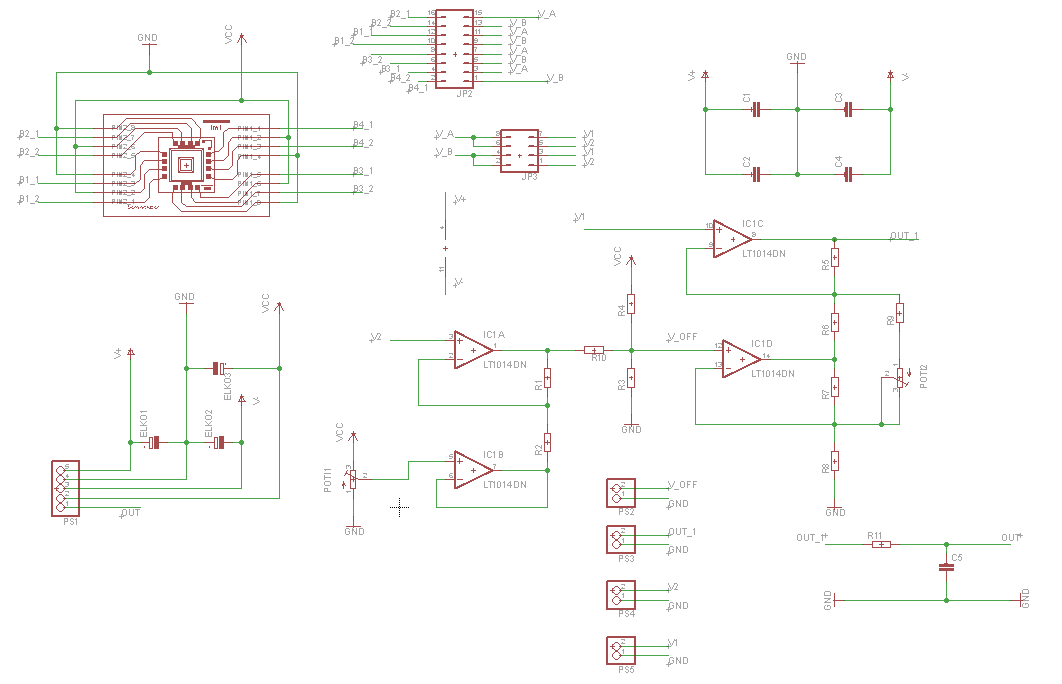
\includegraphics[width=0.9\textwidth]{figures/Auswerteelektronik.PNG}
	\caption{Eagle-Schaltplan der Auswerteelektronik} 
\end{figure}
Im Folgenden wird kurz auf die einzelnen zus�tzlichen Elemente eingegangen.

\subsection{Sensoranschluss}
\label{ssec:1}
Die Eagle-Bibliotheken des IMT beinhalten bereits den grundlegenden Sensoranschluss, deshalb kann dieser direkt daraus �bernommen werden. Beim Wiring ist darauf zu achten, dass sp�ter jede einzelne Br�cke des Sensors separat ausgew�hlt werden kann. Deshalb ben�tigt jede Br�cke eine Verbindung zur Br�ckenspannung (VCC mit 1V) sowie ein Groundpotential. Weiterhin werden pro Br�cke zwei Ausg�nge ben�tigt, die mit der Auswertewerteelektronik zu verbinden sind. Diese dienen also der eigentlichen Druckmessung. In Abbildung \ref{fig:sensoranschluss} sind diese mit Bn\_1 und Bn\_2 beschriftet, wobei n als Br�ckennummer verstanden werden und somit die Werte 1-4 annehmen kann. Die Nummerierung ist dabei frei gew�hlt und hat keine Bedeutung. 
\begin{figure}[h]
	\centering
	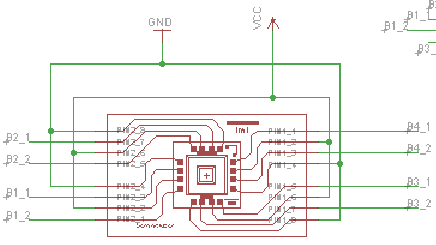
\includegraphics[width=0.7\textwidth]{figures/eagleparts/7_sensorstecker.PNG}
	\caption{Layout Sensoranschluss}\label{fig:sensoranschluss}
\end{figure}
Um die Auswahl einer Br�cke zu erm�glichen, werden die Ausg�nge der Br�cken zun�chst mit einem Jumper mit 8 Eing�ngen verbunden (vgl. Abbildung \ref{fig:jump1}). 
\begin{figure}[h]
	\centering
	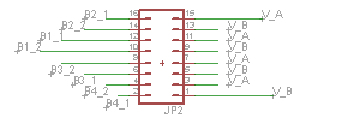
\includegraphics[width=0.6\textwidth]{figures/eagleparts/7_jump1.PNG}
	\caption{Layout Jumper mit Br�ckenausg�ngen als Eingang}\label{fig:jump1}
\end{figure}
Zur Vereinfachung und zur Gew�hrleistung der M�glichkeit des Vertauschens der Eingangspotentiale wird nun ein weiterer Jumper verwendet (vgl. Abbildung \ref{fig:jump2}).
\begin{figure}[h]
	\centering
	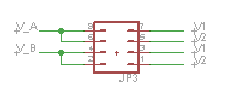
\includegraphics[width=0.5\textwidth]{figures/eagleparts/7_jump2.PNG}
	\caption{Layout Jumper zum Tausch der Eingangspotentiale}\label{fig:jump2}
\end{figure}
Nun kann jede Br�cke individuell ausgew�hlt werden und Eingangspotentiale k�nnen vertauscht werden.

\subsection{Spannungsversorgung}
\label{ssec:2}
Die Versorgung wird durch einen 5-poligen Stecker gew�hrleistet. Neben Groundpotential und Br�ckenspannung (VCC) gibt es noch zwei Eing�nge f�r die Spannungsversorgung der Elektronik (V+ und V-, jeweils bis zu 12V Betragsspannung). �ber OUT wird auf die Messspannung referenziert. Dar�ber hinaus ben�tigt die Baugruppe drei Elektrolytkondensatoren, die zur Stabilisierung dienen. Abbildung \ref{fig:versorgung} zeigt die gesamte Baugruppe.
\begin{figure}[h]
	\centering
	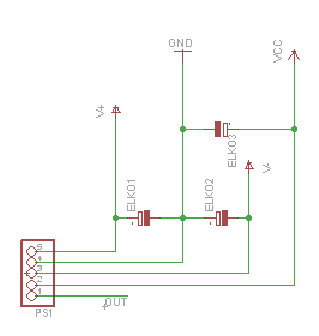
\includegraphics[width=0.5\textwidth]{figures/eagleparts/7_versorgung.PNG}
	\caption{Layout Spannungsversorgung}\label{fig:versorgung}
\end{figure}


\subsection{Spannungsstabilisierung des IC}
\label{ssec:3}
Da der verwendete Operationsverst�rker sehr empfindlich auf Schwankungen seiner Versorgungsspannung sowie auf hochfrequente St�rungen auf den Versorgungsleitungen reagiert, ist es notwendig, diese zu stabilisieren. Dies geschieht �ber eine Baugruppe aus 4 Keramikkondensatoren. Die Funktionsweise �hnelt jener eines Filters. Durch gezieltes Ausnutzen der Be- und Entladezeit der Kondensatoren wird ein einheitliches und konstantes Eingangssignal erreicht. Der Aufbau dieser Spannungsstabilisierung ist in Abbildung \ref{fig:stabic} dargestellt.
\begin{figure}[h]
	\centering
	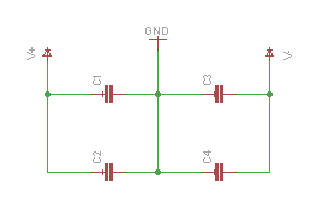
\includegraphics[width=0.5\textwidth]{figures/eagleparts/7_stabilisierungic.PNG}
	\caption{Layout Spannungsstabilisierung Operationsverst�rker}\label{fig:stabic}
\end{figure}

\subsection{Stecker zum Spannungsabgriff}
\label{ssec:4}
Die Messstecker werden f�r eine einfache Kontrolle der Schaltungsspannungen genutzt und an sinnvollen Stellen im Schaltkreis angebracht. Diese sind: \begin{itemize}
\item am Eingangssignal V1
\item am Eingangssignal V2
\item unmittelbar nach der Offsetkompensierung
\item und am Output vor dem RC-Filter.
\end{itemize}
Abbildung \ref{fig:messung} in Verbindung mit Abbildung \ref{fig:Eagle} liefert die Positionen der Messstecker im Schaltplan.
\begin{figure}[h]
	\centering
	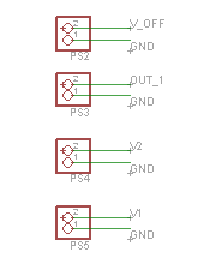
\includegraphics[scale=0.6]{figures/eagleparts/7_messstecker.PNG}
	\caption{Layout Platinenstecker zur Spannungsmessung}\label{fig:messung}
\end{figure}

\section{Platinenlayout (Justus)}
\label{sec:Platinenlayout}
Nachdem der Schaltplan mit Eagle erstellt worden ist, kann in den Board-Editor der Software gewechselt werden. Dieser stellt jegliche Schaltungssymbole als reale Bauteile dar. Die Herausforderung besteht darin, ein sinnvolles Platinenlayout gem�� gewisser Designregeln (vgl. Skript) zu kreieren. Die Platinengr��e muss dabei $5 * 8cm^2$ betragen. Weitere Vorgabe ist die einheitliche Leiterbahnbreite von 3mm und ein Winkel von maximal $45�$. Eine m�gliche L�sung stellt Abbildung \ref{fig:board_justus} dar.
\begin{figure}[h]
	\centering
	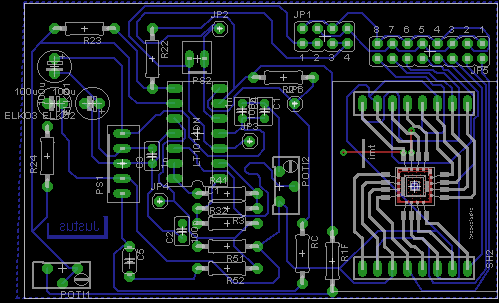
\includegraphics[width=0.7\textwidth]{figures/Board_justus.PNG}
	\caption{M�gliches Platinenlayout}\label{fig:board_justus}
\end{figure}
Abschlie�end sollte die Anordnung �berpr�ft werden. Anschlie�end kann die Platine hergestellt werden.

<<<<<<< HEAD
\section{Platinenerstellung (Justus)}
=======
\section{Designing and Prepration of PCB(Manish kumar)}
For the purpose of designing task we used software called Eagle. It comprises two different editors: the Schematic Editor for the circuit diagram and the Board Editor for the actual PCB. In order to design actual PCB board, we must firstly create our circuit diagram in Schematic Editor. While creating our circuit in Schematic Editor we are using device libraries which contain a wide range of electronic component. This time our circuit must have all additional electronics. RC low-pass filter is needed to filter high frequency noise as long as pressure signals are quasistatic. However, to keep circuit complexity as minimum, the electronics are implemented to measure only one bridge at the time. To ensure that all bridge signals are evaluated, there must be an option to switch between bridges using jumpers. Using our created circuit diagram from Schematic Editor we are creating a concrete PCB layout. In this process, the circuit diagram symbols are replaced with real devices so-called packages. They can be positioned in PCB anywhere. While connecting packages using PCB tracks so-called wires, continuous consistency check is performed on the diagram and layout. After that our next work is preparation of PCB it consists of sereis of operatio which are described below.

\textbf{Printing}
The saved board file was sent for printing as PCB. Since the boards to be printed were small, they were printed aside each other on a mask. The Mask was printed and set to the exposure process.

\textbf{Exposure}
The medium to be printed as the PCB was removed off its protective cover. The printed mask was placed on the medium and exposed to the image-setter for the prescribed time. The main lights were switched off and the medium was immersed into a plastic bowl filled with photographic developer and treated. The board circuits started to appear, whilst the excess layers were removed using sponge. Then the board was readied for the etching process.

\textbf{Etching}
The PCB was then clamped on and set into an etching bath at 40 ? 50oC for 40-50 minutes. The temperature must be monitored as lower temperatures decrease the rate of etching process. A visual examination of the PCB was conducted using LEDs and removed once the etching was completed, to avoid undercutting.

\textbf{Post processing}
Then the PCB was removed off of the photoresistive layers using acetone and the side to be tin-plated was wiped with ethanol. The PCB was then tin-plated to prevent corrosion and blow-dried. A generous coating of conformal coating was applied on the PCB to improve the anti-corrosive property and also to aid soldering. Drills were made on the PCB to allow soldering of the components on the board.

\textbf{Soldering}
The components were soldered on the board according to the schematic and the board design without damaging the board.

\section{Platinenerstellung}
>>>>>>> ad83756170798aaccab44976ac7e8e9f28e431f9
\label{platinenerstellung}
Zur Herstellung wird zun�chst das entworfene Platinenlayout auf eine Maske gedruckt. Diese Maske kann dann auf die Platine, die mit fotosensitiven Lack �berzogen ist, aufgebracht werden. Basismaterial f�r die Platine ist ein Kunststoff. Ist die Maske aufgetragen, folgt die Belichtung und die Entwicklung. Dazu wird die Platine zun�chst f�r zirka 20 Sekunden belichtet und anschlie�end in Natriumpersulfat gebadet. Dort, wo kein Fotolack mehr vorhanden ist (durch Belichtung), greift die �tzl�sung an und es entsteht das gew�nschte Platinendesign. Der �tzvorgang dauert in der Regel 10 bis 40 Minuten, je nach Alter des �tzbades. Ist der �tzvorgang abgeschlossen, muss noch der �brige Fotolack entfernt werden. Dies geschieht mit Hilfe von Aceton. Als finaler Schritt wird die Platine verzinnt, um sie vor Korrosion zu sch�tzen. Abbildung \ref{fig:platine_zinn} zeigt eine fertige Platine, auf die die entsprechenden Bauteile verl�tet werden k�nnen.

\begin{figure}[H]
	\centering
	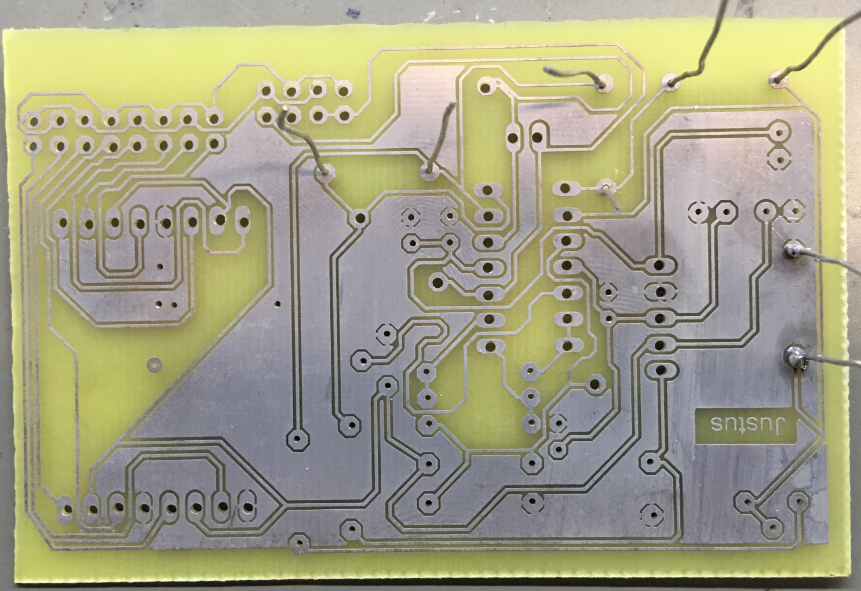
\includegraphics[width=0.7\textwidth]{figures/platine_zinn.PNG}
	\caption{Verzinnte, fertig entwickelte Platine (R�ckseite)}\label{fig:platine_zinn}
\end{figure}

Bevor mit dem L�ten begonnen werden kann, empfiehlt sich die �berpr�fung s�mtlicher Leiterbahnen. Dazu kann ein Multimeter herangezogen werden, welches ein akustisches Signal ausgibt, wenn zwei Punkte, an denen je eine ans Multimeter angeschlossene Elektrode anliegt, miteinander verbunden sind. Beim L�ten muss vor allem darauf geachtet werden, dass weder zu viel noch zu wenig L�tzinn auf die einzelnen L�tstellen aufgetragen wird. Bei falscher Dosierung kann es leicht zu einem Kurzschluss beziehungsweise einer kalten L�tstelle kommen. Abbildung \ref{fig:platine_r} zeigt ein Ergebnis.
\begin{figure}[H]
	\centering
	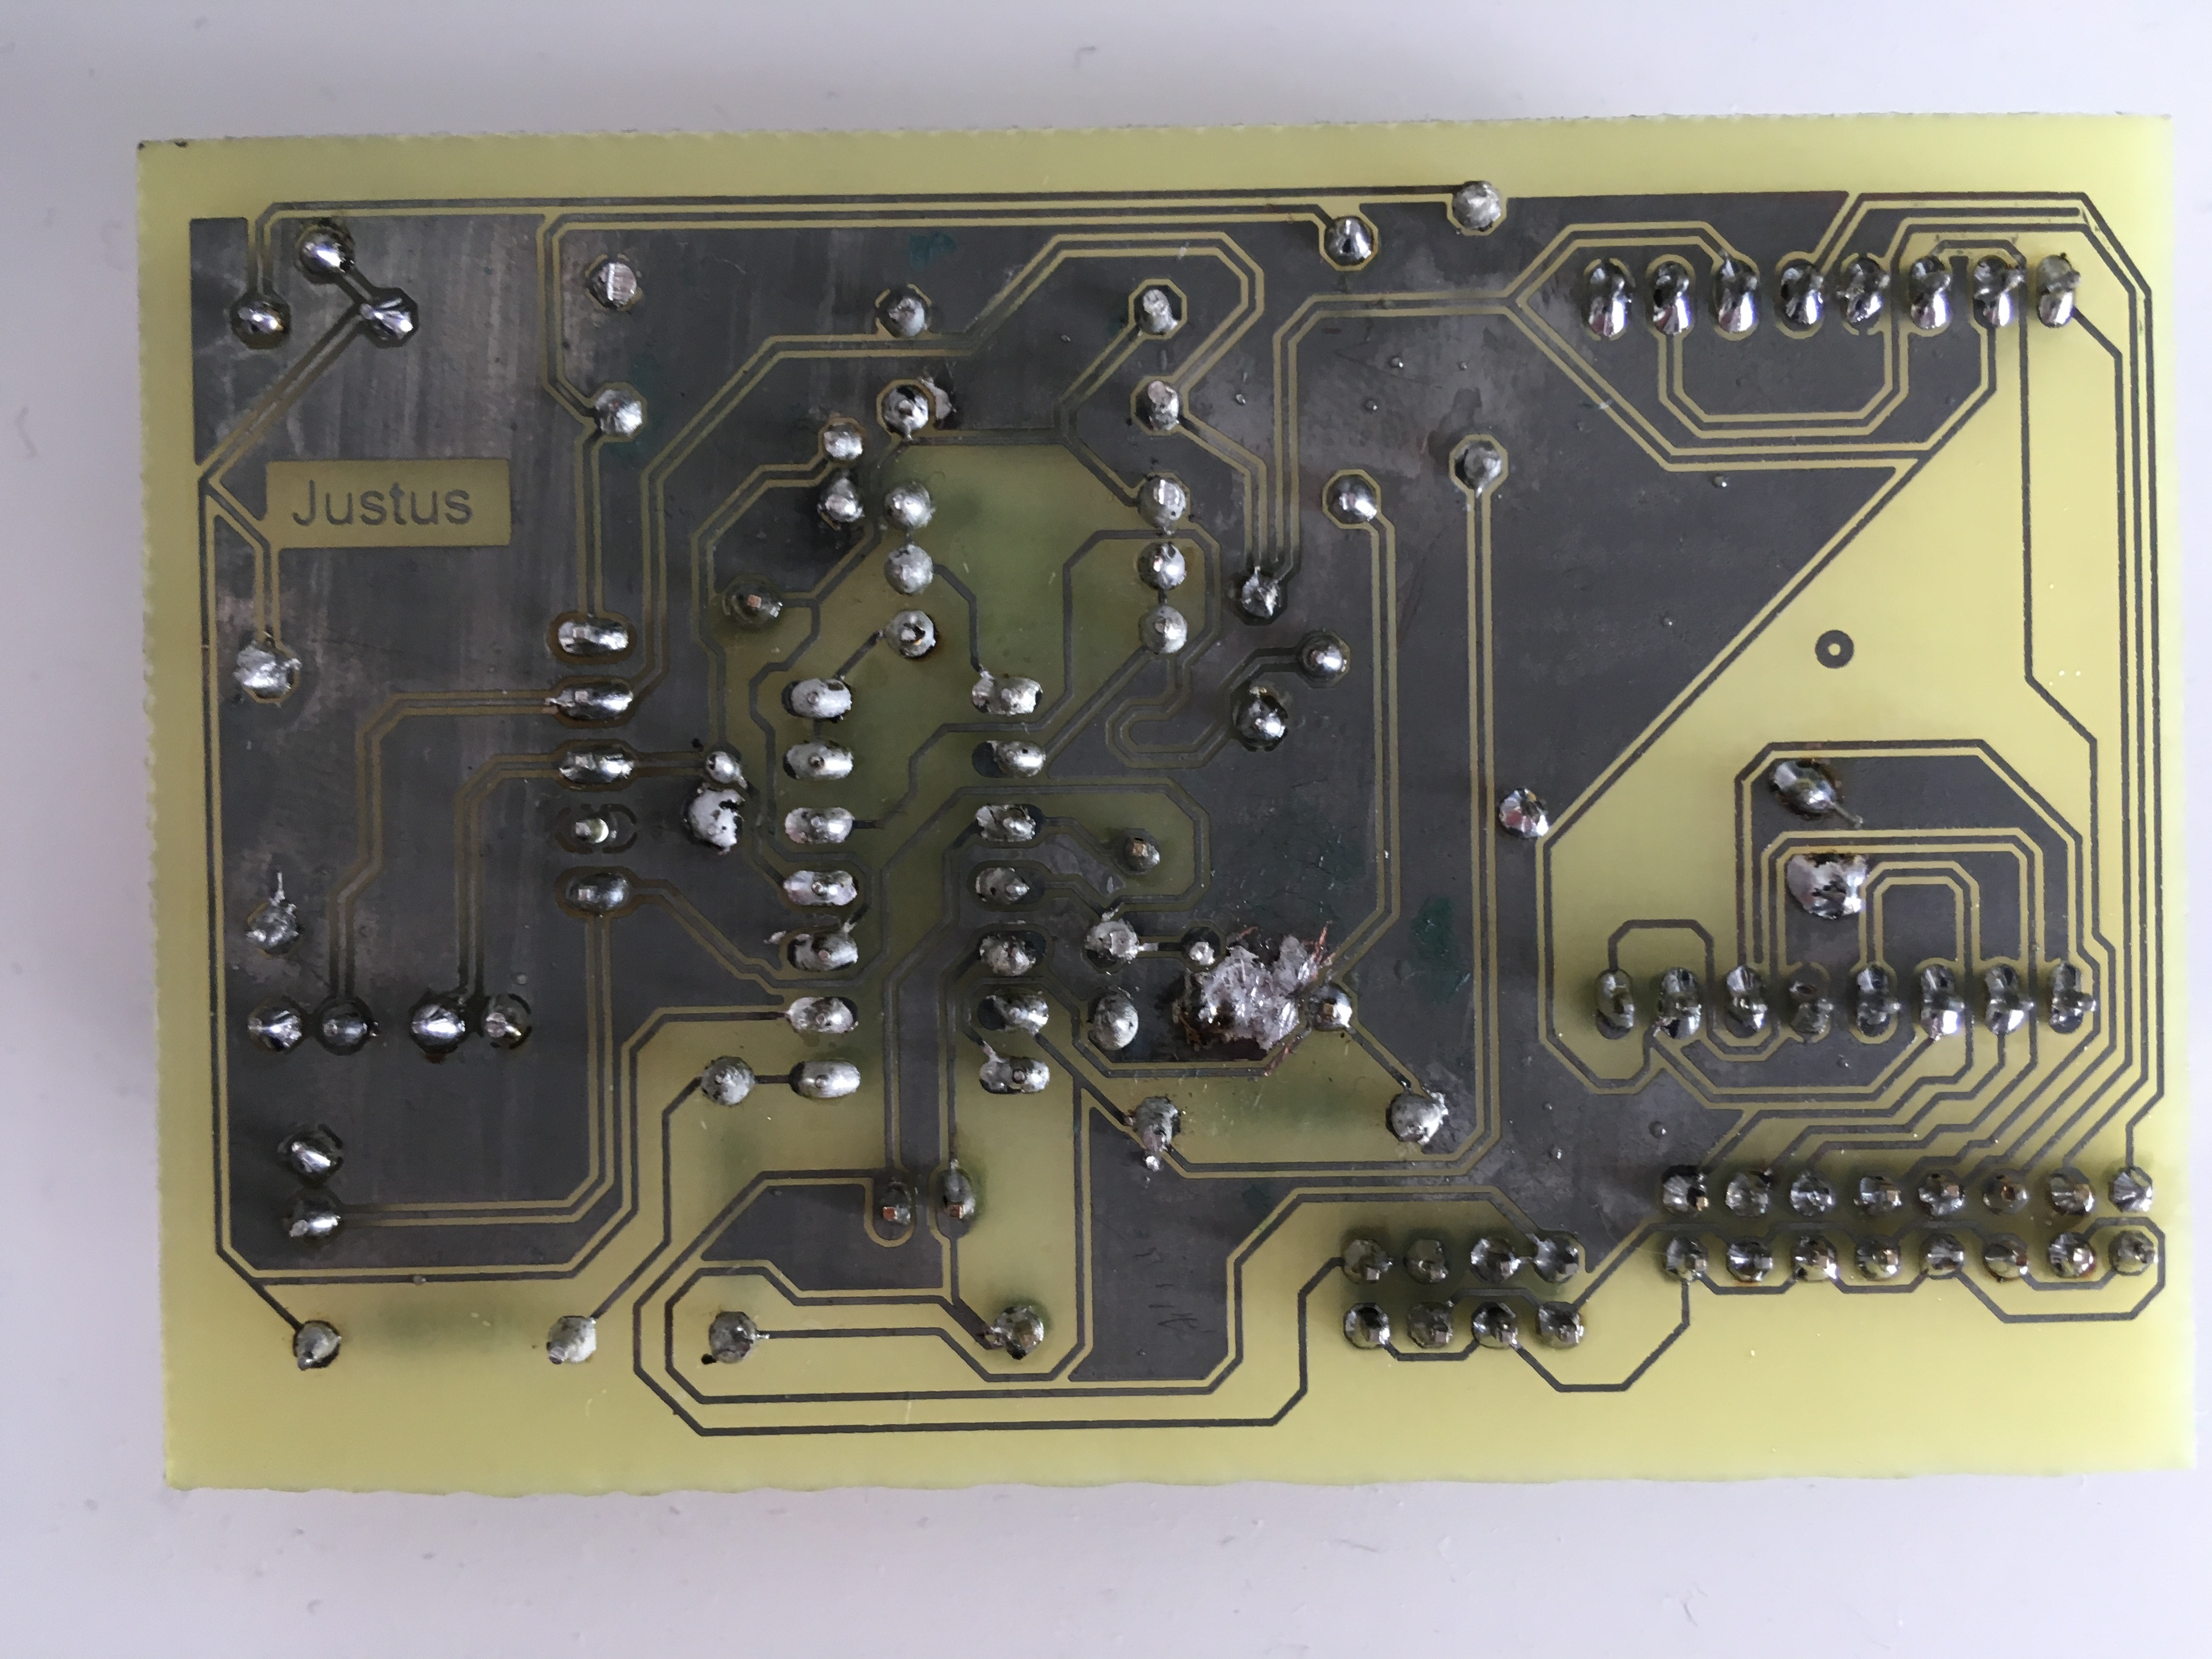
\includegraphics[width=0.7\textwidth]{figures/platine_r.JPG}
	\caption{Fertige Platine R�ckseite}
		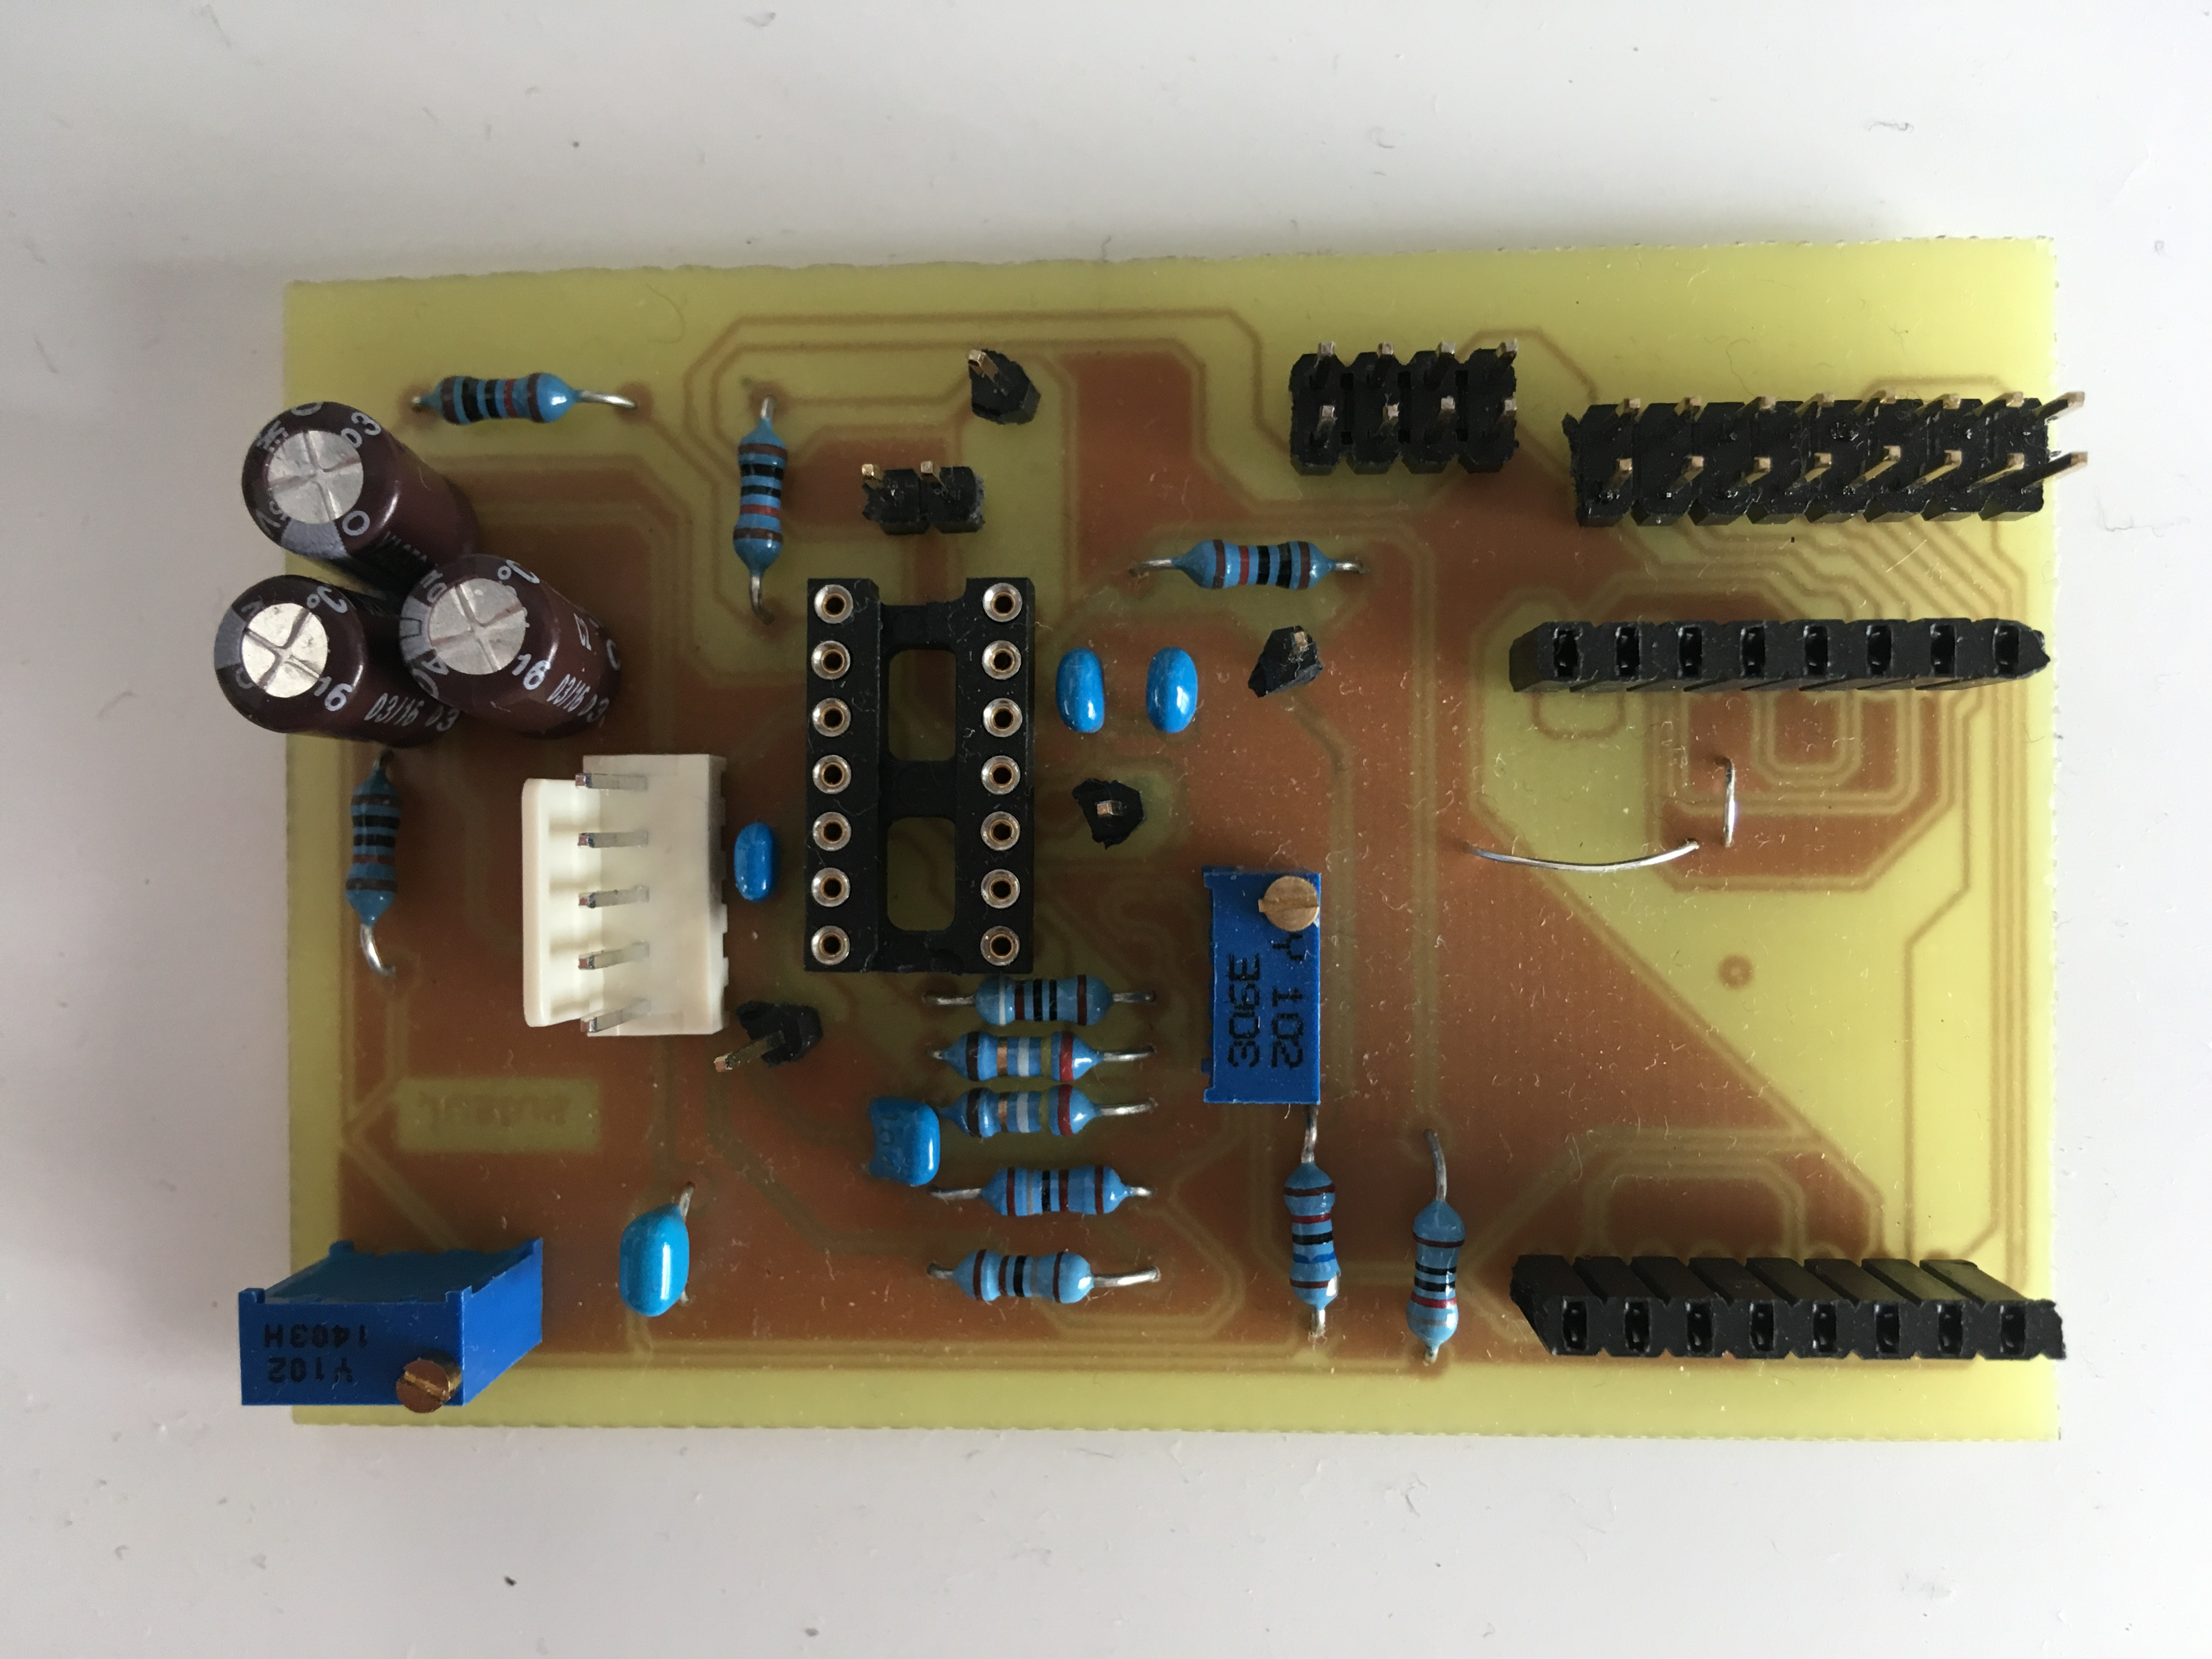
\includegraphics[width=0.7\textwidth]{figures/platine_v.JPG}
	\caption{Fertige Platine Vorderseite}\label{fig:platine_r}
\end{figure}

\section{Evaluation (Manish)}
\label{evaluation}


\begin{figure}[H]
	\centering
	\begin{tikzpicture}\centering
	\begin{axis}[width=0.8\textwidth, xlabel={p / bar},ylabel={U/ mV},legend pos=north west,legend columns=1,xtick distance=0.2]
	\pgfplotstableread{chapters/Daten/Messung.dat}\data
	
	\addplot [color1] table [x=p1,y=V1] {\data};
	\addlegendentry{B1}
	
	\addplot [color2] table [x=p2, y=V2] {\data};
	\addlegendentry{B2}
	
	\addplot [color3] table [x=p3,y=V3] {\data};
	\addlegendentry{B3}
	
	\addplot [color4] table [x=p4,y=V4] {\data};
	\addlegendentry{B4}
	
	\end{axis}
	\end{tikzpicture}
	\caption{Measurement with offset compensation and amplification}\label{pl:Measurments}
\end{figure}
\chapter{Zusammenfassung und Ausblick}
\label{sec:Zusammenfassung}
Hier stehen die Ergebnisse der Arbeit und ein kurzer Ausblick wie es weiter gehen kann.

%=============================== Ende Kapitel =====================================

%\bibliography{chapters/bibliography}              % Literaturverzeichnis

% Anhang (Formatierung)
%\appendix
%\chapter*{Appendix}
%\addcontentsline{toc}{chapter}{appendix}
%\setcounter{chapter}{1}
%\markboth{Anhang}{Anhang}
%\label{Anhang}


%============================ Kapitel des Anhangs ==================================
% Kapitel die als Anhang angef�gt werden sollen

%\section{Morphologischer Kasten}
\label{sec:Anhang_1}

\begin{figure}[h]
	\centering
	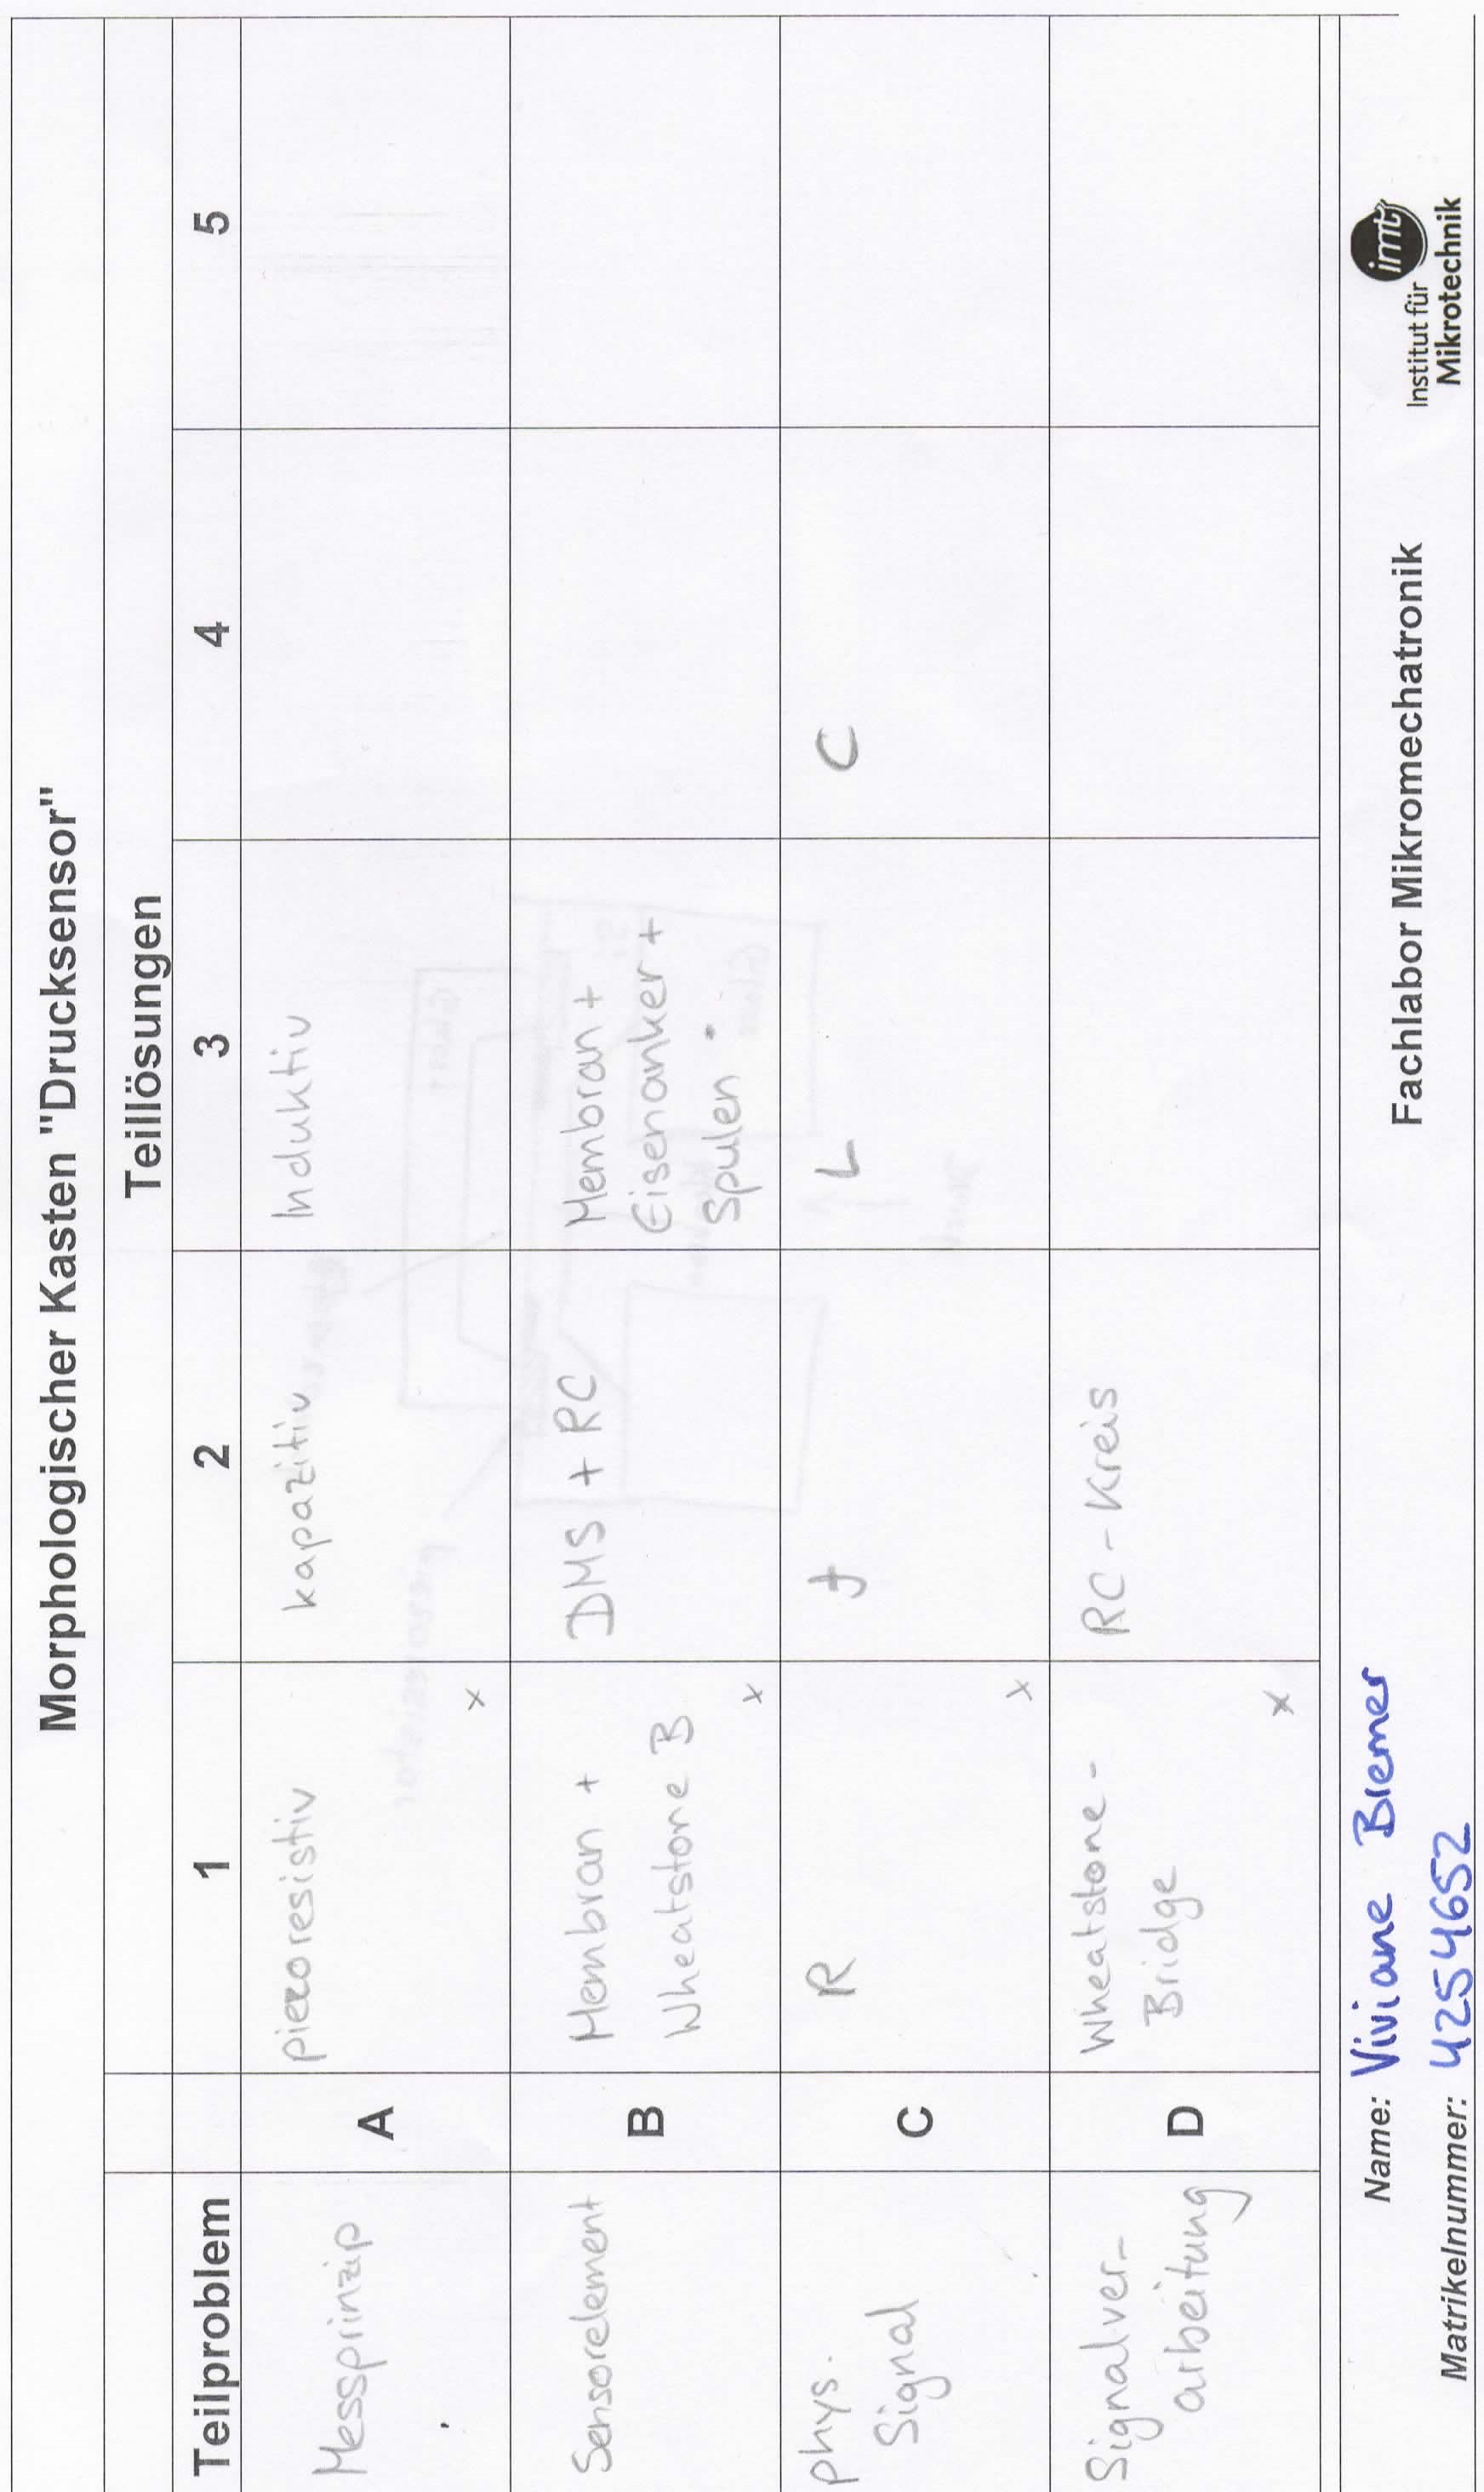
\includegraphics[width=0.7\textwidth]{figures/MorphologischerKasten_Bremer.png}
\end{figure}

\newpage
\section{Anforderungsliste}
\label{sec:Anhang_2}

\begin{figure}[h]
	\centering
	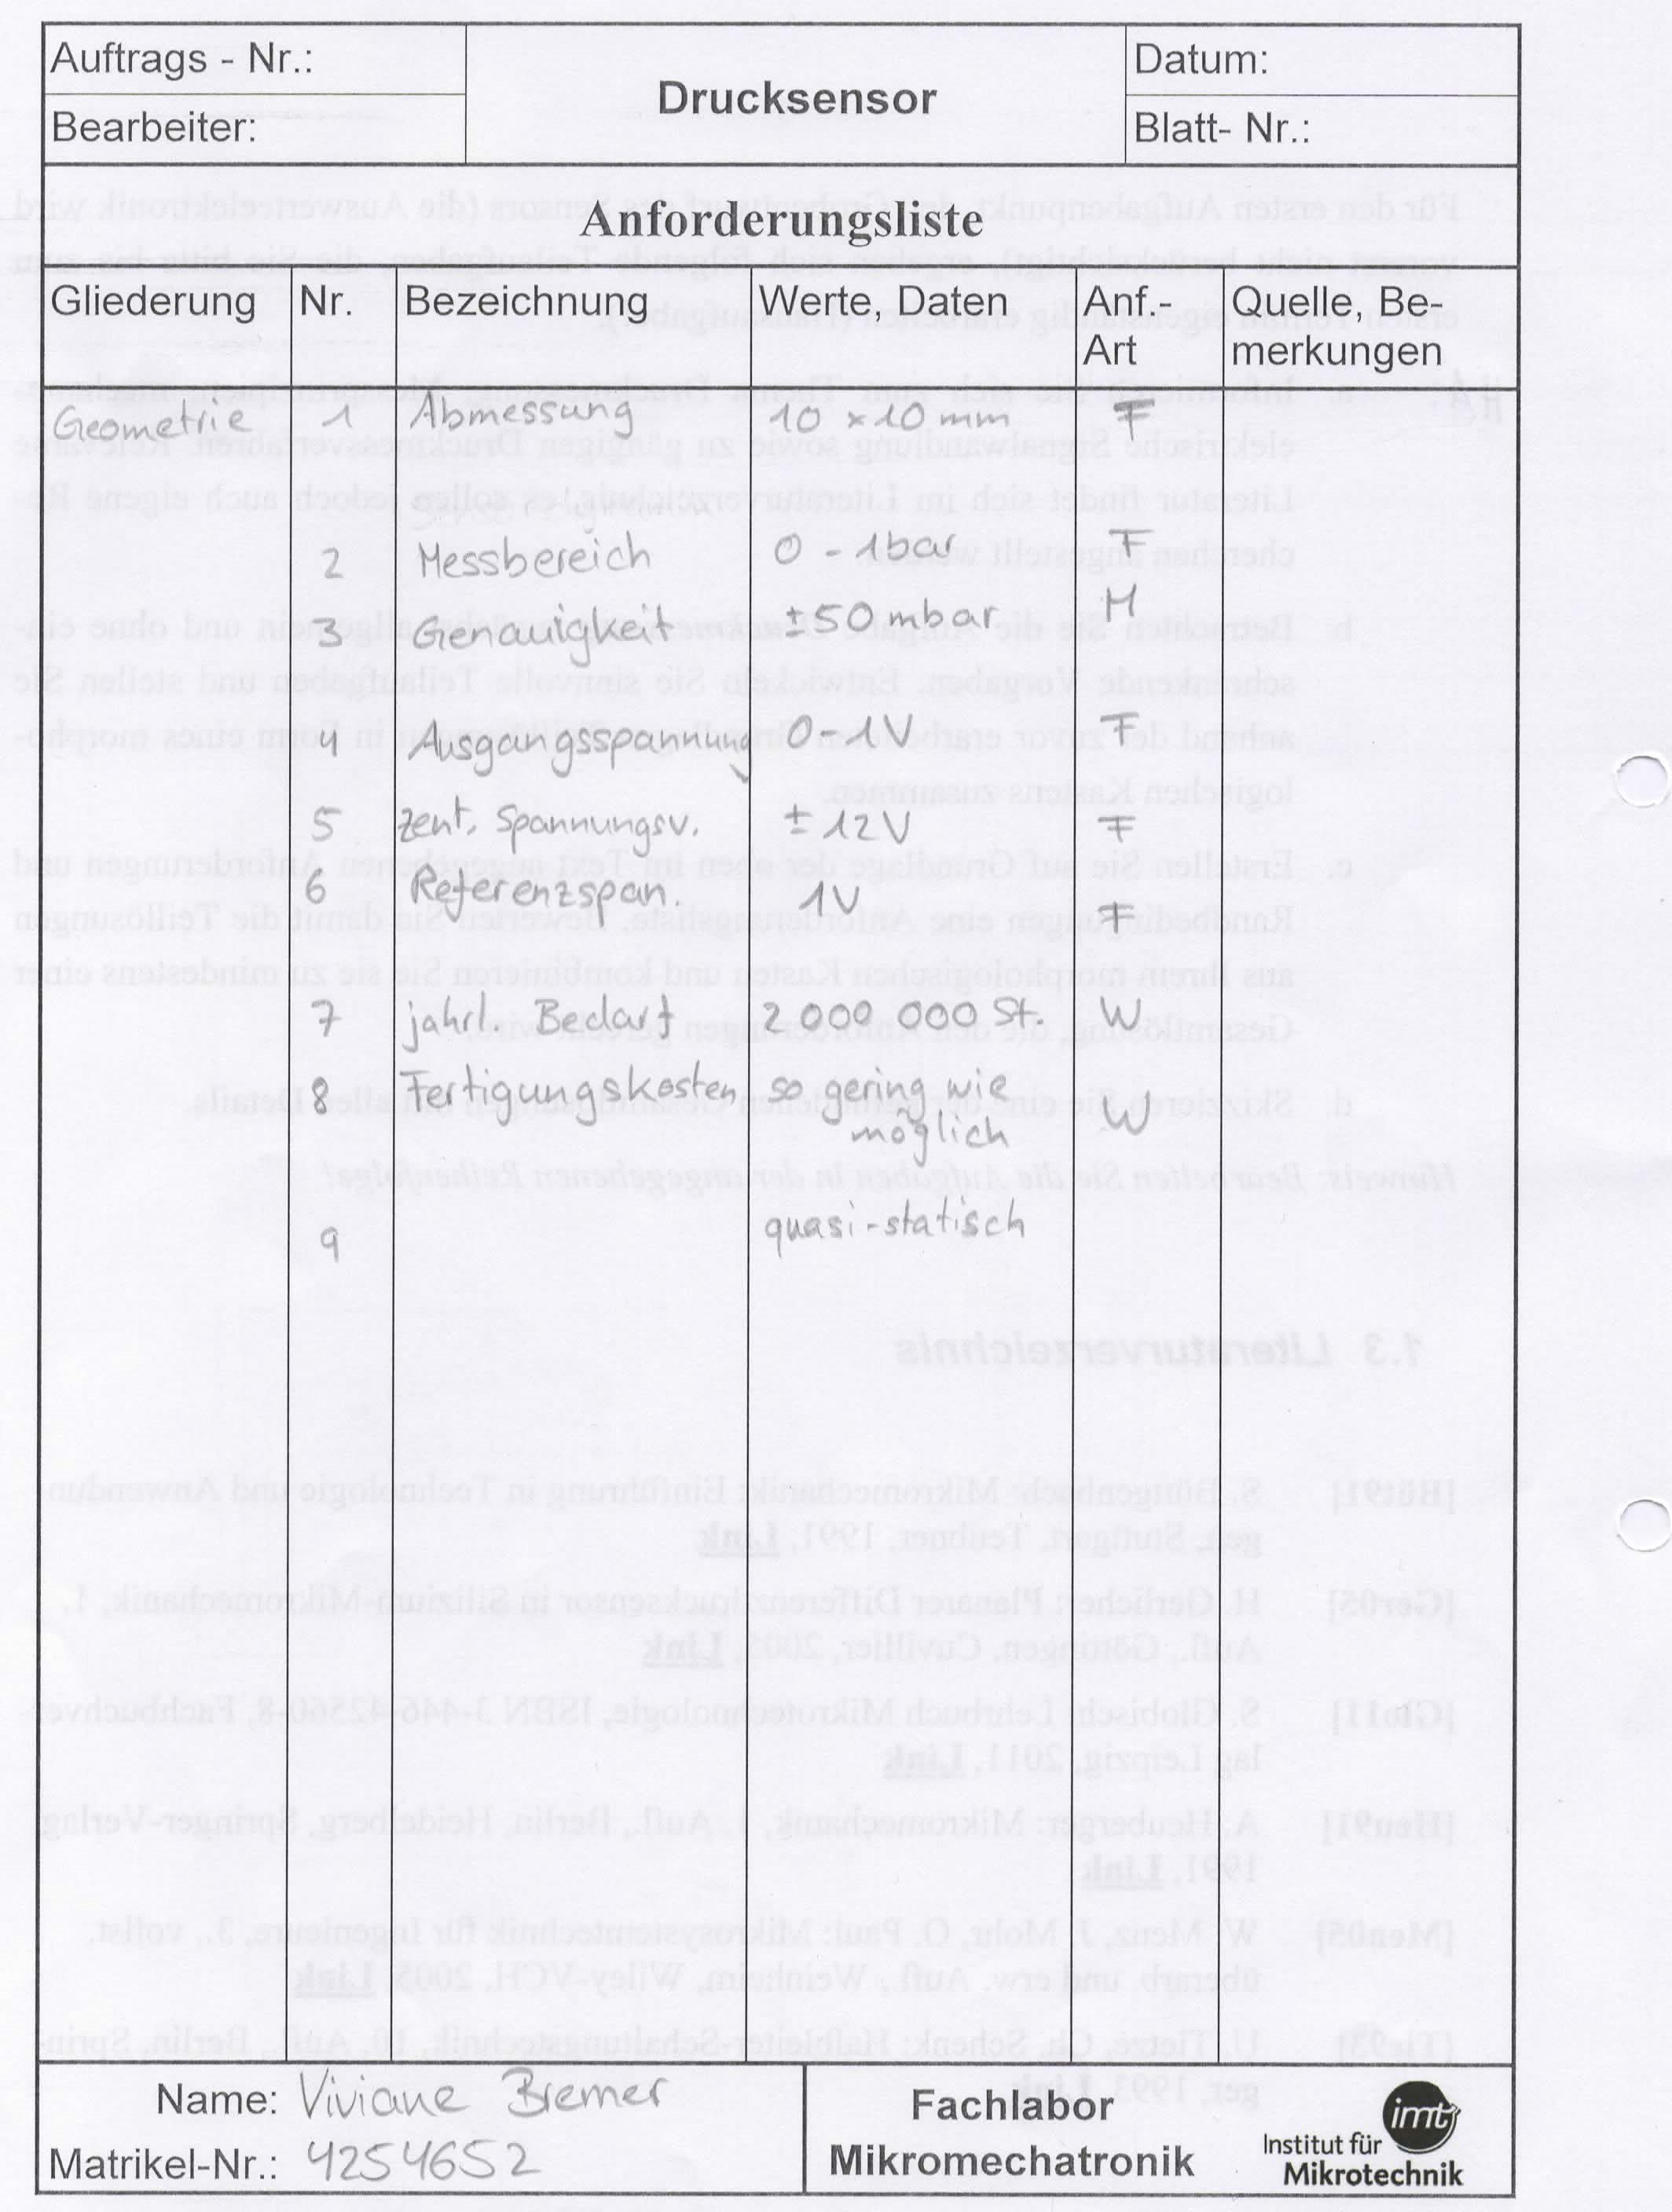
\includegraphics[width=0.9\textwidth]{figures/Anforderungsliste_Bremer.png}
\end{figure}



%================================ Ende Anhangs =====================================


\end{document}                                    % Ende des Dokumentes

